\chapter{Several Variables and Partial Derivatives} \label{pd:chapter}

%%%%%%%%%%%%%%%%%%%%%%%%%%%%%%%%%%%%%%%%%%%%%%%%%%%%%%%%%%%%%%%%%%%%%%%%%%%%%%

\section{Vector spaces, linear mappings, and convexity}
\label{sec:vectorspaces}

\sectionnotes{2--3 lectures}

\subsection{Vector spaces}

The euclidean space $\R^n$ has already made an appearance in the metric
space chapter.  In this chapter, we will extend the differential calculus
we created for one variable to several variables.  The key idea in
differential calculus is to approximate functions by lines and linear
functions.  In several variables we must introduce a little bit of linear
algebra before we can move on.  So
let us start with vector spaces and linear functions on vector spaces.

While it is common to use $\vec{x}$ or the bold
$\mathbf{x}$ for elements of $\R^n$,
especially in the applied sciences,
we use just plain $x$, which is common in mathematics.
That is, $v \in \R^n$ is a \emph{\myindex{vector}}, which means 
$v = (v_1,v_2,\ldots,v_n)$\glsadd{not:vector} is an $n$-tuple of
real numbers.\footnote{Subscripts are used for many purposes,
so sometimes we may have several vectors that may also
be identified by subscript, such as a finite or infinite sequence of
vectors $y_1,y_2,\ldots$.}

It is common to write and treat vectors as
\emph{\myindex{column vectors}}, that is, $n \times 1$ matrices:
%\glsadd{not:vectorcol} FIXME: doesn't seem to work.
\begin{equation*}
v =
(v_1,v_2,\ldots,v_n) =
\mbox{ \scriptsize
$\begin{bmatrix}
v_1 \\ v_2 \\ \vdots \\ v_n
\end{bmatrix}$ }.
\end{equation*}
We will do so when convenient.
We call real numbers
\emph{\myindex{scalars}} to distinguish them from vectors.

The set $\R^n$ has a so-called \emph{vector space} structure defined on it.
However,
even though we will be looking at functions defined on $\R^n$,
not all spaces we wish to deal with are equal to $\R^n$.  Let us
define the abstract notion of the vector space.

\begin{defn}
Let $X$ be a set together with
the operations of addition, $+ \colon X \times X \to X$,
and multiplication, $\cdot \colon \R \times X \to X$, (we usually write $ax$ instead of $a
\cdot x$).  $X$ is called a \emph{\myindex{vector space}} (or a
\emph{\myindex{real vector space}})
if the following conditions are satisfied:
\begin{enumerate}[(i)]
\item (Addition is associative) \quad If $u, v, w \in X$, then $u+(v+w) = (u+v)+w$.
\item (Addition is commutative) \quad If $u, v \in X$, then $u+v = v+u$.
\item (Additive identity) \quad There is a $0 \in X$ such that $v+0=v$ for all $v \in X$.
\item (Additive inverse) \quad For every $v \in X$, there is a $-v \in X$,
such that $v+(-v)=0$.
\item (Distributive law) \quad If $a \in \R$, $u,v \in X$, then
$a(u+v) = au+av$.
\item (Distributive law) \quad If $a,b \in \R$, $v \in X$, then
$(a+b)v = av+bv$.
\item (Multiplication is associative) \quad If $a,b \in \R$, $v \in X$, then
$(ab)v = a(bv)$.
\item (Multiplicative identity) \quad $1v = v$ for all $v \in X$.
\end{enumerate}
Elements of a vector space are usually called \emph{vectors}\index{vector},
even if they
are not elements of $\R^n$ (vectors in the ``traditional'' sense).

If $Y \subset X$ is a subset that is a vector space itself with the same
operations, then $Y$ is called a \emph{\myindex{subspace}} or
a \emph{\myindex{vector subspace}} of $X$.
\end{defn}

\begin{example}
An example vector space is $\R^n$, where addition
and multiplication by a scalar is done componentwise:
if $a \in \R$, $v = (v_1,v_2,\ldots,v_n) \in \R^n$, and $w =
(w_1,w_2,\ldots,w_n) \in \R^n$, then
\begin{align*}
& v+w :=
(v_1,v_2,\ldots,v_n) +
(w_1,w_2,\ldots,w_n) 
=
(v_1+w_1,v_2+w_2,\ldots,v_n+w_n) , \\
& a v :=
a (v_1,v_2,\ldots,v_n) =
(a v_1, a v_2,\ldots, a v_n) .
\end{align*}
\end{example}

In this book we mostly deal with vector spaces that can be often regarded as
subsets of $\R^n$, but there are other vector spaces useful in
analysis.  Let us give a couple of examples.

\begin{example}
A trivial example of a vector space is just
$X := \{ 0 \}$.  The operations are defined in the obvious way: $0 + 0 := 0$
and $a0 := 0$.  A zero vector must always exist,
so all vector spaces are nonempty sets, and this $X$ is in fact the smallest
possible vector space.
\end{example}

\begin{example}
The space $C([0,1],\R)$ of continuous functions on the interval $[0,1]$
is a vector space.  For two functions $f$ and $g$ in $C([0,1],\R)$ and
$a \in \R$, we make the obvious definitions of $f+g$ and $af$:
\begin{equation*}
(f+g)(x) := f(x) + g(x), \qquad (af) (x) := a\bigl(f(x)\bigr) .
\end{equation*}
The 0 is the function that is identically zero.  We leave it as an exercise
to check that all the vector space conditions are satisfied.

The space $C^1([0,1],\R)$ of continuously differentiable functions is
a subspace of $C([0,1],\R)$.
\end{example}

\begin{example}
The space of polynomials $c_0 + c_1 t + c_2 t^2 + \cdots + c_m t^m$
(of arbitrary degree $m$) is a vector space.
Let us denote it by $\R[t]$\glsadd{not:realpoly} (coefficients are real and
the variable is $t$).  The operations are defined in the same way as for
functions above.
Suppose there are
two polynomials, one of degree $m$ and one of degree $n$.  Assume $n
\geq m$ for simplicity.  Then
\begin{multline*}
(c_0 + c_1 t + c_2 t^2 + \cdots + c_m t^m)
+
(d_0 + d_1 t + d_2 t^2 + \cdots + d_n t^n)
= \\
(c_0+d_0) + (c_1+d_1) t + (c_2 + d_2) t^2 + \cdots + (c_m+d_m) t^m
+ d_{m+1} t^{m+1} + \cdots + d_n t^n
\end{multline*}
and
\begin{equation*}
a(c_0 + c_1 t + c_2 t^2 + \cdots + c_m t^m)
=
(ac_0) + (ac_1) t + (ac_2) t^2 + \cdots + (ac_m) t^m  .
\end{equation*}
Despite what it looks like, $\R[t]$ is not equivalent to $\R^n$ for any $n$.  In
particular, it is not ``finite dimensional''.  We will make this notion
precise in just a little bit.  One can make a finite
dimensional vector subspace by restricting the degree.  For example,
if $\sP_n$ is the set of polynomials of degree $n$ or less,
then $\sP_n$ is a finite dimensional vector space, and we could 
identify it with $\R^{n+1}$.

The space $\R[t]$ can be thought of as a subspace of $C(\R,\R)$.  If we
restrict the range of $t$ to $[0,1]$, $\R[t]$ can be identified with
a subspace of $C([0,1],\R)$.
\end{example}

It is often better to think of even simpler ``finite dimensional''
vector spaces using the abstract notion rather than always as $\R^n$.
It is possible to use other fields than $\R$ in the definition (for
example it is common to use the complex numbers $\C$), but let us stick with
the real numbers\footnote{If you want a very funky vector space over a different field,
$\R$ itself is a vector space over the rational numbers.}.

\subsection{Linear combinations and dimension}

\begin{defn}
Suppose $X$ is a vector space,
$x_1, x_2, \ldots, x_k \in X$ are vectors, and
$a_1, a_2, \ldots, a_k \in \R$ are scalars.  Then
\begin{equation*}
a_1 x_1 + 
a_2 x_2 +  \cdots
+ a_k x_k
\end{equation*}
is called a \emph{\myindex{linear combination}} of the vectors $x_1, x_2,
\ldots, x_k$.

If $Y \subset X$ is a set, then the \emph{\myindex{span}} of $Y$, or in notation
$\spn(Y)$, is the set of all linear combinations
of all finite subsets of $Y$.  We also
say $Y$ \emph{\myindex{spans}} $\spn(Y)$\glsadd{not:span}.
\end{defn}

\begin{example}
Let $Y := \{ (1,1) \} \subset \R^2$.  Then
\begin{equation*}
\spn(Y)
=
\{ (x,x) \in \R^2 : x \in \R \} .
\end{equation*}
That is, $\spn(Y)$ is the line through the origin and the point $(1,1)$.
\end{example}

\begin{example} \label{example:vecspr2span}
Let $Y := \{ (1,1), (0,1) \} \subset \R^2$.  Then
\begin{equation*}
\spn(Y)
=
\R^2 ,
\end{equation*}
as any point $(x,y) \in \R^2$ can be written as
a linear combination
\begin{equation*}
(x,y) = x (1,1) + (y-x) (0,1) .
\end{equation*}
\end{example}

\begin{example} \label{example:vecspr2span}
Let $Y := \{ 1, t, t^2, t^3, \ldots \} \subset \R[t]$, and
$E := \{ 1, t^2, t^4, t^6 \ldots \} \subset \R[t]$.

The span of $Y$ is all polynomials,
\begin{equation*}
\spn(Y) = \R[t] .
\end{equation*}
The span of $E$ is the set of polynomials with even powers of $t$ only.
\end{example}

A sum of two linear combinations is again a linear combination, and
a scalar multiple of a linear combination is a linear combination, that is,
\begin{multline*}
(a_1 x_1 + 
a_2 x_2 +  \cdots
+ a_k x_k)
+
(b_1 x_1 + 
b_2 x_2 +  \cdots
+ b_k x_k)
\\
=
(a_1 + b_1) x_1 + 
(a_2 + b_2) x_2 +  \cdots
+ (a_k + b_k) x_k ,
\end{multline*}
and
\begin{equation*}
b (a_1 x_1 + 
a_2 x_2 +  \cdots
+ a_k x_k)
=
b a_1  x_1 + 
b a_2 x_2 +  \cdots
+ b a_k x_k .
\end{equation*}
We formalize this statement in a proposition.

\begin{prop}
Let $X$ be a vector space.  For any $Y \subset X$,
the set $\spn(Y)$ is a vector space itself.
That is, $\spn(Y)$ is a subspace of $X$.
\end{prop}

If $Y$ is already a vector space, then $\spn(Y) = Y$.

\begin{defn}
A set of vectors $\{ x_1, x_2, \ldots, x_k \} \subset X$ is 
\emph{\myindex{linearly independent}}\footnote{%
For an infinite set $Y \subset X$, we would say $Y$ is linearly
independent if every finite subset of $Y$ is linearly independent
in the sense given.
However, this situation only comes up in infinitely many dimensions and
we will not require it.},
if the only solution to
\begin{equation} \label{eq:lincomb}
a_1 x_1 + a_2 x_2 + \cdots + a_k x_k = 0
\end{equation}
is the trivial solution $a_1 = a_2 = \cdots = a_k = 0$.
%Here 0 is the vector of all zeros.
A set that is not linearly independent, is
\emph{\myindex{linearly dependent}}.

A linearly independent set of vectors $B$ such that
$\spn(B) = X$ 
is called a \emph{\myindex{basis}} of $X$.

If a vector space $X$ contains a linearly independent set of $d$ vectors,
but no linearly independent set of $d+1$ vectors, then we say
the \emph{\myindex{dimension}} or $\dim \, X := d$.  If for all $d \in \N$ the vector space
$X$ contains a set of $d$ linearly independent vectors, we say
$X$ is infinite dimensional and write $\dim \, X := \infty$.

For the trivial vector space $\{ 0 \}$, we define $\dim \, \{ 0 \} := 0$.
\end{defn}


For example, the
set $Y$ of the two vectors in
\exampleref{example:vecspr2span} is a basis of $\R^2$, and we have
that $\dim \, \R^2 \geq 2$.
We will see in a moment that any vector subspace of $\R^n$
has a finite dimension, and that dimension is less than or equal to $n$.
It will follow that $\dim \, \R^2 = 2$.

If a set is linearly dependent, then one of the
vectors is a linear combination of the others.  In other words, in
\eqref{eq:lincomb}
if $a_j \not= 0$, then we solve for $x_j$:
\begin{equation*}
x_j = \frac{-a_1}{a_j} x_1 + \cdots + 
\frac{-a_{j-1}}{a_j} x_{j-1} +
\frac{-a_{j+1}}{a_j} x_{j+1} +
\cdots + 
\frac{-a_k}{a_k} x_k .
\end{equation*}
The vector $x_j$ has at least two different representations
as linear combinations of $\{ x_1,x_2,\ldots,x_k \}$. The one above and
$x_j$ itself. 

For example, the set $\{ (0,1), (2,3), (5,0) \}$ is linearly dependent:
\begin{equation*}
3(0,1) - (2,3) + 2(1,0) = 0 ,
\qquad \text{so} \qquad
(2,3) = 3(0,1) + 2(1,0) .
\end{equation*}

\begin{prop}
If $B = \{ x_1, x_2, \ldots, x_k \}$ is a basis of a vector space $X$, then
every point $y \in X$ has a unique representation of the form
\begin{equation*}
y = \sum_{j=1}^k a_j \, x_j
\end{equation*}
for some scalars $a_1, a_2, \ldots, a_k$.
\end{prop}

\begin{proof}
Every $y \in X$ is a linear combination of elements of $B$
since $X$ is the span of $B$.  For uniqueness
suppose
\begin{equation*}
y = \sum_{j=1}^k a_j x_j = \sum_{j=1}^k b_j x_j ,
\end{equation*}
then
\begin{equation*}
\sum_{j=1}^k (a_j-b_j) x_j = 0 .
\end{equation*}
By linear independence of the basis $a_j = b_j$ for all $j$.
\end{proof}

For $\R^n$
we define
\begin{equation*}
e_1 := (1,0,0,\ldots,0) , \quad
e_2 := (0,1,0,\ldots,0) , \quad \ldots, \quad
e_n := (0,0,0,\ldots,1) ,
\end{equation*}
and call this the \emph{\myindex{standard basis}} of $\R^n$.\glsadd{not:standardbasis}
We use the same letters $e_j$ for any $\R^n$, and
which space $\R^n$ we are working in is understood from context.
A direct computation shows that $\{ e_1, e_2, \ldots, e_n \}$ is really
a basis of $\R^n$; it spans $\R^n$ and is
linearly independent.  In fact,
\begin{equation*}
x = (x_1,x_2,\ldots,x_n) = \sum_{j=1}^n x_j e_j .
\end{equation*}

\begin{prop} \label{mv:dimprop}
%(\textbf{(Theorems 9.2 and 9.3 in Rudin):})
Let $X$ be a vector space and $d$ a nonnegative integer.
\begin{enumerate}[(i)]
\item \label{mv:dimprop:i}
If $X$ is spanned by $d$ vectors, then $\dim \, X \leq d$.
\item \label{mv:dimprop:ii}
$\dim \, X = d$ if and only if $X$ has a basis of $d$
vectors (and so every basis has $d$ vectors).
\item \label{mv:dimprop:iii}
In particular, $\dim \, \R^n = n$.
\item \label{mv:dimprop:iv}
If $Y \subset X$ is a vector subspace and $\dim \, X = d$,
then $\dim \, Y \leq d$.
\item \label{mv:dimprop:v}
If $\dim \, X = d$ and a set $T$ of $d$ vectors spans $X$,
then $T$ is linearly independent.
\item \label{mv:dimprop:vi}
If $\dim \, X = d$ and a set $T$ of $m$ vectors is
linearly independent, then there is a set $S$ of $d-m$
vectors such that $T \cup S$ is a basis of $X$.
\end{enumerate}
\end{prop}

\begin{proof}
Let us start with \ref{mv:dimprop:i}.
Suppose $S = \{ x_1 , x_2, \ldots, x_d \}$ spans $X$, and
$T = \{ y_1, y_2, \ldots, y_m \}$ is a set of linearly independent
vectors of $X$.  We wish to show that $m \leq d$.
Write
\begin{equation*}
y_1 = \sum_{k=1}^d a_{k,1} x_k ,
\end{equation*}
for some numbers $a_{1,1},a_{2,1},\ldots,a_{d,1}$,
which we can do as $S$ spans $X$.  One of the
$a_{k,1}$ is nonzero (otherwise $y_1$ would be zero),
so suppose without loss of generality that this
is $a_{1,1}$.  Then we solve
\begin{equation*}
x_1 = \frac{1}{a_{1,1}} y_1 - \sum_{k=2}^d \frac{a_{k,1}}{a_{1,1}} x_k .
\end{equation*}
In particular, $\{ y_1 , x_2, \ldots, x_d \}$ span $X$, since $x_1$ can be
obtained from $\{ y_1 , x_2, \ldots, x_d \}$.  Therefore, there are some numbers
for some numbers $a_{1,2},a_{2,2},\ldots,a_{d,2}$, such that
\begin{equation*}
y_2 = a_{1,2} y_1 + \sum_{k=2}^d a_{k,2} x_k .
\end{equation*}
As $T$ is linearly independent, one of the $a_{k,2}$
for $k \geq 2$ must be nonzero.  Without loss of generality suppose 
$a_{2,2} \not= 0$.  Proceed to solve for 
\begin{equation*}
x_2 = \frac{1}{a_{2,2}} y_2 - \frac{a_{1,2}}{a_{2,2}} y_1 - \sum_{k=3}^d
\frac{a_{k,2}}{a_{2,2}} x_k .
\end{equation*}
In particular,
$\{ y_1 , y_2, x_3, \ldots, x_d \}$ spans $X$.
%The astute reader will think back to linear algebra and notice that we are
%row-reducing a matrix.

We continue this procedure.  If $m < d$, then we are done.  So suppose
$m \geq d$.
After $d$ steps we obtain that 
$\{ y_1 , y_2, \ldots, y_d \}$ spans $X$.  Any
other vector $v$ in $X$ is a linear combination of
$\{ y_1 , y_2, \ldots, y_d \}$, and hence cannot be in $T$ as $T$ is
linearly independent.  So $m = d$.

Let us look at \ref{mv:dimprop:ii}.
First, if $T$ is a set of $k$ linearly independent vectors
that do not span $X$, that is $X \setminus
\spn (T) \not= \emptyset$, then choose a vector $v \in X \setminus
\spn (T)$.  The set $T \cup \{ v \}$ is linearly independent (exercise).
If $\dim \, X = d$,
then there must exist some linearly independent set of $d$ vectors $T$,
and it must span $X$, otherwise we could choose a larger set of linearly
independent vectors.  So we have a basis of $d$ vectors.
On the other hand if we have a basis of $d$ vectors,
it is linearly independent and spans $X$ by definition.  By \ref{mv:dimprop:i} we know
there is no set of $d+1$ linearly independent vectors, so dimension must be $d$.

For \ref{mv:dimprop:iii} notice that $\{ e_1, e_2, \ldots, e_n \}$ is a basis of $\R^n$.

To see \ref{mv:dimprop:iv},
suppose $Y$ is a vector space and $Y \subset X$,
where $\dim \, X = d$.  As $X$ cannot contain $d+1$ linearly independent
vectors, neither can $Y$.

For \ref{mv:dimprop:v} suppose $T$ is a set of $m$ vectors that is linearly dependent
and spans $X$.  Then one of the
vectors is a linear combination of the others.  Therefore, if we remove it
from $T$ we obtain a set of $m-1$ vectors that still span $X$ and hence
$\dim \, X \leq m-1$ by \ref{mv:dimprop:i}.

For \ref{mv:dimprop:vi} suppose $T = \{ x_1, x_2, \ldots, x_m \}$ is
a linearly independent set.  We follow the procedure above in the proof of
\ref{mv:dimprop:ii}
to keep adding vectors while keeping the set linearly independent.
As the dimension is $d$ we can add a vector exactly $d-m$ times.
\end{proof}

\subsection{Linear mappings}

A function $f \colon X \to Y$, when $Y$ is not $\R$, is often called a
\emph{\myindex{mapping}} or a \emph{\myindex{map}}
rather than a \emph{function}.
%  The word
%function is then usually reserved for the case $Y=\R$.


\begin{defn}
A mapping $A \colon X \to Y$ of vector spaces $X$ and $Y$
is \emph{\myindex{linear}} (or a
\emph{\myindex{linear transformation}})
if for every $a \in \R$ and every $x,y \in X$,
\begin{equation*}
A(a x) = a A(x), \qquad \text{and} \qquad A(x+y) = A(x)+A(y) .
\end{equation*}
We usually write $Ax$ instead of $A(x)$ if $A$ is linear.
If $A$ is one-to-one and onto, then we say $A$ is
\emph{invertible}\index{invertible linear transformation},
and we denote the inverse by $A^{-1}$.
If $A \colon X \to X$ is linear, then we say $A$ is a
\emph{\myindex{linear operator}} on $X$.

We write $L(X,Y)$\glsadd{not:LXY} for the set of all linear transformations from $X$ to
$Y$, and just $L(X)$\glsadd{not:LX} for the set of linear operators on $X$.
If $a \in \R$ and $A,B \in L(X,Y)$, define
the transformations $aA$ and $A+B$ by
\begin{equation*}
(aA)(x) := aAx ,
\qquad
(A+B)(x) := Ax + Bx .
\end{equation*}

If $A \in L(Y,Z)$ and $B \in L(X,Y)$, define the
transformation $AB$ as the composition $A \circ B$, that is,
\begin{equation*}
ABx := A(Bx) .
\end{equation*}

Finally denote by $I \in L(X)$ the \emph{\myindex{identity}}: 
the linear operator such that $Ix = x$ for all $x$.
\end{defn}

It is not hard to see that $aA \in L(X,Y)$
and $A+B \in L(X,Y)$, and that $AB \in L(X,Z)$.
In particular, $L(X,Y)$ is a vector space.
As the set $L(X)$ is not only a vector space, but also
admits a product (composition of operators),
it is often called an \emph{\myindex{algebra}}.

An immediate consequence of the definition of a linear mapping is: if
$A$ is linear, then $A0 = 0$.

\begin{prop}
If $A \in L(X,Y)$ is invertible, then $A^{-1}$ is linear.
\end{prop}

\begin{proof}
Let $a \in \R$ and $y \in Y$.  As $A$ is onto, then there is an 
$x$ such that $y = Ax$, and further as it is also one-to-one
$A^{-1}(Az) = z$ for all $z \in X$.  So
\begin{equation*}
A^{-1}(ay)
=
A^{-1}(aAx)
=
A^{-1}\bigl(A(ax)\bigr)
= ax
= aA^{-1}(y).
\end{equation*}
Similarly let $y_1,y_2 \in Y$, and $x_1, x_2 \in X$ such that
$Ax_1 = y_1$ and 
$Ax_2 = y_2$, then
\begin{equation*}
A^{-1}(y_1+y_2)
=
A^{-1}(Ax_1+Ax_2)
=
A^{-1}\bigl(A(x_1+x_2)\bigr)
= x_1+x_2
= A^{-1}(y_1) + A^{-1}(y_2). \qedhere
\end{equation*}
\end{proof}

\begin{prop} \label{mv:lindefonbasis}
If $A \in L(X,Y)$ is linear, then it is completely determined
by its values on a basis of $X$.
Furthermore, if $B$ is a basis of $X$,
then any function $\widetilde{A} \colon B \to Y$ extends to a linear
function on $X$.
\end{prop}

We will only prove this proposition for finite dimensional spaces, as we do
not need infinite dimensional spaces.
For infinite dimensional spaces, the proof is essentially the same, but a
little trickier to write, so let us stick with finitely many dimensions.

\begin{proof}
Let $\{ x_1, x_2, \ldots, x_n \}$ be a basis and suppose 
$A x_j = y_j$.  Every $x \in X$ has a unique representation
\begin{equation*}
x = \sum_{j=1}^n b_j \, x_j
\end{equation*}
for some numbers $b_1,b_2,\ldots,b_n$.  By linearity
\begin{equation*}
Ax = 
A\sum_{j=1}^n b_j x_j
=
\sum_{j=1}^n b_j \, Ax_j
=
\sum_{j=1}^n b_j \, y_j .
\end{equation*}
The ``furthermore'' follows by setting $y_j := \widetilde{A}(x_j)$,
and defining the extension as
$Ax := \sum_{j=1}^n b_j y_j$.  The function is well defined by
uniqueness of the representation of $x$.
We leave it to the reader to check that $A$ is linear.
\end{proof}

The next proposition only works for finite dimensional vector spaces.
It is a special case of the so-called rank-nullity theorem from linear
algebra.

%\textbf{Theorem 9.5:}
\begin{prop} \label{mv:prop:lin11onto}
If $X$ is a finite dimensional vector space and $A \in L(X)$, then $A$ is one-to-one if and only if it is onto.
\end{prop}

\begin{proof}
Let $\{ x_1,x_2,\ldots,x_n \}$ be a basis for $X$.
Suppose $A$ is one-to-one.  Now suppose
\begin{equation*}
\sum_{j=1}^n c_j \, Ax_j =
A\sum_{j=1}^n c_j \, x_j =
0 .
\end{equation*}
As $A$ is one-to-one,
the only vector that is taken to 0 is 0 itself.  
Hence,
\begin{equation*}
0 =
\sum_{j=1}^n c_j x_j
\end{equation*}
and $c_j = 0$ for all $j$.
So $\{ Ax_1, Ax_2, \ldots, Ax_n \}$ is a linearly independent set.
By \propref{mv:dimprop}
and the fact that the dimension is $n$, we conclude
$\{ Ax_1, Ax_2, \ldots, Ax_n \}$ span $X$.  Any point $x \in X$
can be written as
\begin{equation*}
x = \sum_{j=1}^n a_j \, Ax_j =
A\sum_{j=1}^n a_j \, x_j ,
\end{equation*}
so $A$ is onto.

Now suppose $A$ is onto.  As $A$ is determined by the action on
the basis we see that every element of $X$ has to be in the span of
$\{ Ax_1, Ax_2, \ldots, Ax_n \}$.  Suppose 
\begin{equation*}
A\sum_{j=1}^n c_j \, x_j =
\sum_{j=1}^n c_j \, Ax_j = 0 .
\end{equation*}
By \propref{mv:dimprop}
as $\{ Ax_1, Ax_2, \ldots, Ax_n \}$ span $X$, the set is independent,
and hence $c_j = 0$ for all $j$.  In other words if $Ax = 0$, then $x=0$.  This means that
$A$ is one-to-one:  If $Ax = Ay$, then $A(x-y) = 0$ and so
$x=y$.
\end{proof}

We leave the proof of the next proposition as an exercise.

\begin{prop} \label{prop:LXYfinitedim}
If $X$ and $Y$ are finite dimensional vector spaces, then $L(X,Y)$
is also finite dimensional.
\end{prop}

Finally let us note that we often identify a finite dimensional vector
space $X$ of dimension $n$ with $\R^n$, provided we fix a basis $\{ x_1,
x_2, \ldots, x_n \}$ in $X$.  That is, we define a bijective
linear map $A \in L(X,\R^n)$ by
$Ax_j = e_j$, where $\{ e_1, e_2, \ldots, e_n \}$.  Then we have
the correspondence
\begin{equation*}
\sum_{j=1}^n c_j \, x_j \, \in X
\quad
\overset{A}{\mapsto}
\quad
(c_1,c_2,\ldots,c_n) \, \in \R^n .
\end{equation*}

\subsection{Convexity}

A subset $U$ of a vector space is \emph{\myindex{convex}}
if whenever $x,y \in U$, the line segment from
$x$ to $y$ lies in $U$.  That is, if the \emph{\myindex{convex combination}}
$(1-t)x+ty$ is in $U$ for all $t \in [0,1]$.  See \figureref{mv:convexcomb}.

\begin{myfigureht}
\subimport*{figures/}{convexset.pdf_t}
\caption{Convexity.\label{mv:convexcomb}}
\end{myfigureht}

In $\R$, convex sets are precisely the intervals.
In $\R^2$ (or higher
dimensions) there are lots of nonconvex connected sets.  For example
the set $\R^2 \setminus \{0\}$ is not convex but it is connected.  To see
this simply take any $x \in \R^2 \setminus \{0\}$ and let $y:=-x$.
Then $(\nicefrac{1}{2})x + (\nicefrac{1}{2})y = 0$, which is not in the set.
On the other hand, the ball $B(x,r) \subset \R^n$ (using the standard metric
on $\R^n$)
is convex by the triangle inequality.

\begin{exercise}
Show that in $\R^n$ any ball $B(x,r)$ for $x \in \R^n$ and $r > 0$ is
convex.
\end{exercise}

\begin{example}
As a convex combination is in particular a linear combination,
any subspace $V$ of a vector space $X$ is convex.
\end{example}

\begin{example}
A somewhat more complicated example is given by the following.  Let
$C([0,1],\R)$ be the vector space of continuous real valued functions on $\R$.
Let $X \subset C([0,1],\R)$ be the set of those $f$ such that
\begin{equation*}
\int_0^1 f(x)~dx \leq 1 \qquad \text{and} \qquad
f(x) \geq 0 \text{ for all $x \in [0,1]$} .
\end{equation*}
Then $X$ is convex.  Take $t \in [0,1]$, and note that if $f,g \in X$,
then $t f(x) + (1-t) g(x) \geq 0$ for all $x$.  Furthermore
\begin{equation*}
\int_0^1 \bigl(tf(x) + (1-t)g(x)\bigr) ~dx
=
t \int_0^1 f(x) ~dx
+ (1-t)\int_0^1 g(x) ~dx \leq 1 .
\end{equation*}
Note that $X$ is not a subspace of $C([0,1],\R)$.
\end{example}

\begin{prop}
The intersection two convex sets is convex.  In fact,
if $\{ C_\lambda \}_{\lambda \in I}$ is
an arbitrary collection of convex sets, then
\begin{equation*}
C := \bigcap_{\lambda \in I} C_\lambda
\end{equation*}
is convex.
\end{prop}

\begin{proof}
If $x, y \in C$, then $x,y \in C_\lambda$ for all
$\lambda \in I$, and hence if $t \in [0,1]$, then $tx + (1-t)y \in
C_\lambda$ for all $\lambda \in I$.  Therefore, $tx + (1-t)y \in C$ and $C$
is convex.
\end{proof}

\begin{prop}
Let $T \colon V \to W$ be a linear mapping between two vector spaces and
let $C \subset V$ be a convex set.  Then $T(C)$ is convex.
\end{prop}

\begin{proof}
Take any two points $p,q \in T(C)$.  Pick $x,y \in C$ such that
$Tx = p$ and $Ty=q$.  As $C$ is convex, then
$tx+(1-t)y \in C$
for all $t \in [0,1]$, so
\begin{equation*}
tp+(1-t)q 
=
tTx+(1-t)Ty
=
T\bigl(tx+(1-t)y\bigr)
\in T(C) .  \qedhere
\end{equation*}
\end{proof}

For completeness, a very useful construction is the
\emph{\myindex{convex hull}}.  Given any set $S \subset V$ of a vector
space, define the convex hull of $S$, by
\begin{equation*}
\operatorname{co}(S) :=
\bigcap \{ C \subset V : S \subset C, \text{ and $C$ is convex} \} .
\end{equation*}
That is, the convex hull is the smallest convex set containing $S$.  
By a proposition above, the intersection of convex sets is convex and
hence, the convex hull is convex.

\begin{example}
The convex hull of 0 and 1 in $\R$ is $[0,1]$.  Proof:
Any convex set containing 0 and 1 must contain $[0,1]$.  The set $[0,1]$
is convex, therefore it must be the convex hull.
\end{example}

\subsection{Exercises}

\begin{exercise}
Verify that $\R^n$ is a vector space.
\end{exercise}

\begin{exercise}
Let $X$ be a vector space.
Prove that a finite set of vectors $\{ x_1,x_2,\ldots,x_n \} \subset X$ 
is linearly independent if and only if for every $j=1,2,\ldots,n$
\begin{equation*}
\spn( \{ x_1,\ldots,x_{j-1},x_{j+1},\ldots,x_n \}) \subsetneq
\spn( \{ x_1,x_2,\ldots,x_n \}) .
\end{equation*}
That is, the span of the set with one vector removed is strictly smaller.
\end{exercise}

\begin{exercise}
Show that the set $X \subset C([0,1],\R)$ of those functions such 
that $\int_0^1 f = 0$ is a vector subspace.
\end{exercise}

\begin{exercise}[Challenging]
Prove $C([0,1],\R)$ is an infinite dimensional vector space
where the operations are defined in the obvious way:
$s=f+g$ and $m=fg$ are defined as
$s(x) := f(x)+g(x)$ and
$m(x) := f(x)g(x)$.
Hint: for the dimension, think of functions that are only nonzero
on the interval $(\nicefrac{1}{n+1},\nicefrac{1}{n})$.
\end{exercise}

\begin{exercise}
Let $k \colon [0,1]^2 \to \R$ be continuous.  Show that
$L \colon C([0,1],\R) \to C([0,1],\R)$ defined by
\begin{equation*}
Lf(y) := \int_0^1 k(x,y)f(x)~dx
\end{equation*}
is a linear operator.  That is, show that $L$ is well defined (that
$Lf$ is continuous), and that $L$ is linear.
\end{exercise}

\begin{exercise}
Let $\sP_n$ be the vector space of polynomials in one variable of degree $n$
or less.  Show that $\sP_n$ is a vector space of dimension $n+1$.
\end{exercise}

\begin{exercise}
Let $\R[t]$ be the vector space of polynomials in one variable $t$.  Let
$D \colon \R[t] \to \R[t]$ be the derivative operator (derivative in $t$).
Show that $D$ is a linear operator.
\end{exercise}

\begin{exercise}
Let us show that \propref{mv:prop:lin11onto} only works in finite
dimensions.  Take $\R[t]$ and define the operator $A \colon \R[t] \to \R[t]$
by $A\bigl(P(t)\bigr) = tP(t)$.  Show that $A$ is linear and one-to-one, but
show that it is not onto.
\end{exercise}

\begin{exercise}
Finish the proof of \propref{mv:lindefonbasis} in the finite dimensional case.
That is, suppose,
$\{ x_1, x_2,\ldots x_n \}$ is a basis of $X$,
$\{ y_1, y_2,\ldots y_n \} \subset Y$ and we define a
function
\begin{equation*}
Ax := \sum_{j=1}^n b_j y_j, \qquad \text{if} \quad x=\sum_{j=1}^n b_j x_j .
\end{equation*}
Then prove that $A \colon X \to Y$ is linear.
\end{exercise}


\begin{exercise}
Prove \propref{prop:LXYfinitedim}.  Hint: A linear operator is determined by
its action on a basis.  So given two bases
$\{ x_1,\ldots,x_n \}$ and
$\{ y_1,\ldots,y_m \}$ for $X$ and $Y$ respectively, consider the linear
operators $A_{jk}$ that send $A_{jk} x_j = y_k$, and 
$A_{jk} x_\ell = 0$ if $\ell \not= j$.
\end{exercise}

\begin{exercise}[Easy]
Suppose $X$ and $Y$ are vector spaces and $A \in L(X,Y)$ is a linear
operator.\\
a) Show that the nullspace $N := \{ x \in X : Ax = 0 \}$ is a
vectorspace.
\\
b) Show that the range $R := \{ y \in Y : Ax = y \text{ for some $x \in X$} \}$ is a
vectorspace.
\end{exercise}

\begin{exercise}[Easy]
Show by example that a union of convex sets need not be convex.
\end{exercise}

\begin{exercise}
Compute the convex hull of the set of 3 points $\{ (0,0), (0,1), (1,1) \}$ in
$\R^2$.
\end{exercise}

\begin{exercise}
Show that the set $\{ (x,y) \in \R^2 : y > x^2 \}$ is a convex set.
\end{exercise}

\begin{exercise}
Show that the set $X \subset C([0,1],\R)$ of those functions such 
that $\int_0^1 f = 1$ is a convex set, but not a vector subspace.
\end{exercise}


\begin{exercise}
Show that every convex set in $\R^n$ is connected using the standard
topology on $\R^n$.
\end{exercise}

\begin{exercise}
Suppose $K \subset \R^2$ is a convex set such that the only point of
the form $(x,0)$ in $K$ is the point $(0,0)$.  Further suppose that
there $(0,1) \in K$ and $(1,1) \in K$.  Then show that if $(x,y) \in K$,
then $y > 0$ unless $x=0$.
\end{exercise}

%%%%%%%%%%%%%%%%%%%%%%%%%%%%%%%%%%%%%%%%%%%%%%%%%%%%%%%%%%%%%%%%%%%%%%%%%%%%%%

\sectionnewpage
\section{Analysis with vector spaces}
\label{sec:normsmatsdets}

\sectionnotes{2-3 lectures}

\subsection{Norms}

Let us start measuring distance.

\begin{defn}
If $X$ is a vector space, then we say
a function $\snorm{\cdot} \colon X \to \R$ is a
\emph{\myindex{norm}}\glsadd{not:norm} if:
\begin{enumerate}[(i)]
\item \label{defn:norm:i} $\snorm{x} \geq 0$, with $\snorm{x}=0$ if and only if $x=0$.
\item \label{defn:norm:ii} $\snorm{cx} = \abs{c}\snorm{x}$ for all $c \in \R$ and $x \in X$.
\item \label{defn:norm:iii} $\snorm{x+y} \leq \snorm{x}+\snorm{y}$ for all $x,y \in X$
\qquad (Triangle inequality)\index{triangle inequality for norms}.
\end{enumerate}
\end{defn}

Before defining the standard norm on $\R^n$, let us
define the standard 
scalar \emph{\myindex{dot product}} on $\R^n$.  For two vectors
if $x=(x_1,x_2,\ldots,x_n) \in \R^n$
and $y=(y_1,y_2,\ldots,y_n) \in \R^n$, define\glsadd{not:dotprod}
\begin{equation*}
x \cdot y := \sum_{j=1}^n x_j y_j .
\end{equation*}
It is easy to see that the dot product is linear in each variable
separately.  That is,
if $y$ is fixed the map $x \mapsto x \cdot y$ is linear map from
$\R^n$ to $\R$.  Similarly, if $x$ is fixed, then
$y \mapsto x \cdot y$ is also linear.
The \emph{\myindex{Euclidean norm}} is defined as\glsadd{not:normRn}
\begin{equation*}
\snorm{x} := \snorm{x}_{\R^n} := \sqrt{x \cdot x} = \sqrt{(x_1)^2+(x_2)^2 + \cdots + (x_n)^2}.
\end{equation*}
We normally just use $\snorm{x}$, but sometimes it will be necessary to
emphasize that we are talking about the euclidean norm and use
$\snorm{x}_{\R^n}$.
It is easy to see that the Euclidean norm satisfies \ref{defn:norm:i} and
\ref{defn:norm:ii}.  To prove
that \ref{defn:norm:iii} holds, the key
inequality is the so-called Cauchy--Schwarz inequality
we saw before.  As this inequality is so important let us restate and
reprove it using the notation of this chapter.

\begin{thm}[\myindex{Cauchy--Schwarz inequality}]
Let $x, y \in \R^n$, then
\begin{equation*}
\abs{x \cdot y} \leq \snorm{x}\snorm{y} = \sqrt{x\cdot x}\, \sqrt{y\cdot y},
\end{equation*}
with equality if and only if the vectors are scalar multiples of each other.
\end{thm}

\begin{proof}
If $x=0$ or $y = 0$, then the theorem holds trivially.
So assume $x\not= 0$ and $y \not= 0$.

If $x$ is a scalar multiple of $y$, that is $x = \lambda y$ for some
$\lambda \in \R$, then the theorem holds with equality:
\begin{equation*}
\abs{\lambda y \cdot y} = \abs{\lambda} \, \abs{y\cdot y} =
\abs{\lambda} \, \snorm{y}^2 = \snorm{\lambda y} \snorm{y} .
\end{equation*}

Next take $x+ty$, we find that
$\snorm{x+ty}^2$ is a quadratic polynomial in $t$:
\begin{equation*}
\snorm{x+ty}^2 =
(x+ty) \cdot (x+ty) =
x \cdot x + x \cdot ty + ty \cdot x + ty \cdot ty
=
\snorm{x}^2 + 2t(x \cdot y) + t^2 \snorm{y}^2 .
\end{equation*}
If $x$ is not a scalar multiple of $y$, then 
$\snorm{x+ty}^2 > 0$ for all $t$.  So the polynomial $\snorm{x+ty}^2$
is never zero.
Elementary algebra says that the discriminant must be negative:
\begin{equation*}
4 {(x \cdot y)}^2 - 4 \snorm{x}^2\snorm{y}^2 < 0,
\end{equation*}
or in other words ${(x \cdot y)}^2 < \snorm{x}^2\snorm{y}^2$.
\end{proof}

Item \ref{defn:norm:iii}, the triangle inequality in $\R^n$,
follows via the following computation:
\begin{equation*}
\snorm{x+y}^2 
=
x \cdot x + y \cdot y + 2 (x \cdot y)
\leq
\snorm{x}^2 + \snorm{y}^2 + 2 (\snorm{x}\snorm{y})
=
{(\snorm{x} + \snorm{y})}^2 .
\end{equation*}

The distance
$d(x,y) := \snorm{x-y}$ is the standard
distance (standard metric) on $\R^n$ that
we used when we talked about metric spaces.

On any vector space $X$, once we
have a norm (any norm),
we define a distance $d(x,y) := \snorm{x-y}$, and this
$d$ makes $X$ into
a metric space (an easy exercise).

%Let $A \in L(\R^n,\R^m)$.  Define
\begin{defn}
Let $A \in L(X,Y)$.  Define
\begin{equation*}
\snorm{A} :=
\sup \{ \snorm{Ax} : x \in X ~ \text{with} ~ \snorm{x} = 1 \} .
\end{equation*}
The number $\snorm{A}$ is called the \emph{\myindex{operator norm}}.  We will see below
that indeed it is a norm (at least for finite dimensional spaces).
Again, when necessary to emphasize which norm we are talking about, we may
write it as $\snorm{A}_{L(X,Y)}$.\glsadd{not:normLXY}
\end{defn}

By linearity,
$\norm{A \frac{x}{\snorm{x}}} = \frac{\snorm{Ax}}{\snorm{x}}$,
for any nonzero $x \in X$.
The vector $\frac{x}{\snorm{x}}$ is of norm 1.
Therefore,
\begin{equation*}
\snorm{A} =
\sup \{ \snorm{Ax} : x \in X ~ \text{with} ~ \snorm{x} = 1 \}
=
\sup_{\substack{x \in X\\x\neq 0}} \frac{\snorm{Ax}}{\snorm{x}} .
\end{equation*}
This implies that
\begin{equation*}
\snorm{Ax} \leq \snorm{A}  \snorm{x} .
\end{equation*}
%although the inequality may be strict.  For example,
%Suppose that on $\R^2$, $A(1,0) = (0,0)$ and
%$A(0,1) = (0,1)$.  Then it is not hard to FIXME?

It is not hard to see from the definition that $\snorm{A} = 0$ if and
only if $A = 0$, that is, if $A$ takes every vector to the zero vector.

It is also not difficult to see the norm of the identity operator:
\begin{equation*}
\snorm{I} =
\sup_{\substack{x \in X\\x\neq 0}} \frac{\snorm{Ix}}{\snorm{x}} 
=
\sup_{\substack{x \in X\\x\neq 0}} \frac{\snorm{x}}{\snorm{x}} 
= 1.
\end{equation*}

For finite dimensional spaces, $\snorm{A}$ is always finite as we prove
below.  This also implies that $A$ is continuous.
For infinite dimensional spaces neither statement needs to be true.  For a simple
example,
take the vector space of continuously differentiable functions on $[0,1]$
and as the norm use the uniform norm.  The functions
$\sin(nx)$ have norm 1, but the derivatives have norm $n$.  So
differentiation (which is a linear operator) has unbounded norm on this
space.  But let us stick to finite dimensional spaces now.

When we talk about finite dimensional vector space, one often thinks of
$\R^n$, although if we have a norm, the norm might perhaps not be
the standard euclidean norm.  In the exercises, you can prove that
every norm is ``equivalent'' to the euclidean norm in that the
topology it generates is the same.  For simplicity, we only prove the
following proposition for the euclidean space, and the proof for a general
finite dimensional space is left as an exercise.

\begin{prop} \label{prop:finitedimpropnormfin}
Let $X$ and $Y$ be finite dimensional vector spaces with a norm.
If $A \in L(X,Y)$, then $\snorm{A} < \infty$, and
$A$ is uniformly continuous (Lipschitz with constant $\snorm{A}$).
\end{prop}

\begin{proof}
As we said we only prove the proposition for euclidean space so suppose
that $X = \R^n$ and $Y=\R^m$ and the norm is the standard euclidean norm.
The general case is left as an exercise.

Let $\{ e_1,e_2,\ldots,e_n \}$ be the standard basis of $\R^n$.
Write $x \in \R^n$, with $\snorm{x} = 1$, as
\begin{equation*}
x = \sum_{j=1}^n c_j e_j .
\end{equation*}
Since $e_j \cdot e_\ell = 0$ whenever $j\not=\ell$ and $e_j \cdot e_j = 1$,
then $c_j = x \cdot e_j$ and
\begin{equation*}
\abs{c_j} = \abs{ x \cdot e_j }
\leq \snorm{x} \snorm{e_j} = 1 .
\end{equation*}
Then
\begin{equation*}
\snorm{Ax} =
\norm{\sum_{j=1}^n c_j Ae_j}
\leq
\sum_{j=1}^n \abs{c_j} \snorm{Ae_j} 
\leq
\sum_{j=1}^n \snorm{Ae_j} .
\end{equation*}
The right hand side does not depend on $x$.  We found
a finite upper bound independent of $x$, so $\snorm{A} < \infty$.

For any vector spaces $X$ and $Y$, and $A \in L(X,Y)$, suppose that
$\snorm{A} < \infty$.
For $v,w \in X$,
\begin{equation*}
\snorm{A(v-w)} \leq \snorm{A} \snorm{v-w} .
\end{equation*}
As $\snorm{A} < \infty$, then this says $A$ is Lipschitz with constant $\snorm{A}$.
\end{proof}

\begin{prop} \label{prop:finitedimpropnorm}
Let $X$, $Y$, and $Z$ be finite dimensional vector spaces with a norm.
{\ }
%\textbf{Proposition (Theorem 9.7 in Rudin):}
\begin{enumerate}[(i)]
\item \label{item:finitedimpropnorm:i}
If $A,B \in L(X,Y)$ and $c \in \R$, then
\begin{equation*}
\snorm{A+B} \leq \snorm{A}+\snorm{B}, \qquad \snorm{cA} = \abs{c}\snorm{A} .
\end{equation*}
In particular, the operator norm is a norm on the vector space $L(X,Y)$.
\item \label{item:finitedimpropnorm:ii}
If $A \in L(X,Y)$ and $B \in L(Y,Z)$, then
\begin{equation*}
\snorm{BA} \leq \snorm{B} \snorm{A} .
\end{equation*}
\end{enumerate}
\end{prop}

\begin{proof}
For \ref{item:finitedimpropnorm:i},
\begin{equation*}
\snorm{(A+B)x} =
\snorm{Ax+Bx} \leq
\snorm{Ax}+\snorm{Bx} \leq
\snorm{A} \snorm{x}+\snorm{B}\snorm{x} =
(\snorm{A}+\snorm{B}) \snorm{x} .
\end{equation*}
So $\snorm{A+B} \leq \snorm{A}+\snorm{B}$.

Similarly,
\begin{equation*}
\snorm{(cA)x} =
\abs{c} \snorm{Ax} \leq (\abs{c}\snorm{A}) \snorm{x} .
\end{equation*}
Thus $\snorm{cA} \leq \abs{c}\snorm{A}$.  Next,
\begin{equation*}
\abs{c} \snorm{Ax}
=
\snorm{cAx} \leq \snorm{cA} \snorm{x} .
\end{equation*}
Hence $\abs{c}\snorm{A} \leq \snorm{cA}$.

For \ref{item:finitedimpropnorm:ii} write
\begin{equation*}
\snorm{BAx} \leq \snorm{B} \snorm{Ax} \leq \snorm{B} \snorm{A} \snorm{x} .
\qedhere
\end{equation*}
\end{proof}

As a norm defines a metric,
there is
a metric space topology on $L(X,Y)$, so we can talk
about open/closed sets, continuity, and convergence.

%\textbf{Theorem 9.8:}
\begin{prop} \label{prop:finitedimpropinv}
Let $X$ be a finite dimensional vector space with a norm.
Let $U \subset L(X)$ be the set of invertible linear operators.
\begin{enumerate}[(i)]
\item \label{finitedimpropinv:i}
If $A \in U$ and $B \in L(X)$, and
\begin{equation} \label{eqcontineq}
\snorm{A-B} <  \frac{1}{\snorm{A^{-1}}},
\end{equation}
then $B$ is invertible.
\item \label{finitedimpropinv:ii}
$U$ is open and $A \mapsto A^{-1}$ is a continuous
function on $U$.
\end{enumerate}
\end{prop}

Let us make sense of this on a simple example.
Think back to $\R^1$, where linear operators are just
numbers $a$ and the operator norm of $a$ is simply $\abs{a}$.
The operator $a$ is invertible ($a^{-1} = \nicefrac{1}{a}$)
whenever $a \not=0$.  The condition $\abs{a-b} < \frac{1}{\abs{a^{-1}}}$ does
indeed imply that $b$ is not zero.  And $a \mapsto \nicefrac{1}{a}$ is a continuous
map.
When $n > 1$, then there are other noninvertible operators than just zero,
and in general things are a bit more difficult.

\begin{proof}
Let us prove \ref{finitedimpropinv:i}.   We know something about $A^{-1}$
and something about $A-B$.  These are linear operators so let us
apply them to a vector.
\begin{equation*}
A^{-1}(A-B)x
=
x-A^{-1}Bx .
\end{equation*}
Therefore,
\begin{equation*}
\begin{split}
\snorm{x} 
& =
\snorm{A^{-1} (A-B)x + A^{-1}Bx}
\\
& \leq
\snorm{A^{-1}}\snorm{A-B} \snorm{x} + \snorm{A^{-1}}\snorm{Bx} .
\end{split}
\end{equation*}
% First a straight forward computation
%\begin{equation*}
%\begin{split}
%\snorm{x} =
%\snorm{A^{-1}Ax}
%& \leq
%\snorm{A^{-1}} \snorm{Ax}
%\\
%& \leq
%\snorm{A^{-1}} ( \snorm{(A-B)x} + \snorm{Bx} )
%\\
%& \leq
%\snorm{A^{-1}}\snorm{A-B} \snorm{x} + \snorm{A^{-1}}\snorm{Bx} .
%\end{split}
%\end{equation*}
Now assume $x \neq 0$ and so $\snorm{x} \neq 0$.
Using \eqref{eqcontineq} we obtain
\begin{equation*}
\snorm{x} < \snorm{x} + \snorm{A^{-1}}\snorm{Bx} ,
\end{equation*}
or in other words $\snorm{Bx} \not= 0$ for all nonzero $x$, and hence
$Bx \not= 0$ for all nonzero $x$.  This is enough to see that
$B$ is one-to-one (if $Bx = By$, then $B(x-y) = 0$, so $x=y$).
As $B$ is one-to-one operator from $X$ to $X$ which is finite dimensional
and hence is invertible.

Let us look at \ref{finitedimpropinv:ii}.  Fix some $A \in U$.  Let $B$ be invertible and near $A$,
that is $\snorm{A-B} \snorm{A^{-1}} <  \nicefrac{1}{2}$.
Then \eqref{eqcontineq} is satisfied.
We have shown above (using $B^{-1}y$ instead of $x$)
\begin{equation*}
\snorm{B^{-1}y} \leq 
\snorm{A^{-1}}\snorm{A-B} \snorm{B^{-1}y} + \snorm{A^{-1}}\snorm{y}
\leq
\nicefrac{1}{2} \snorm{B^{-1}y} + \snorm{A^{-1}}\snorm{y} ,
\end{equation*}
or
\begin{equation*}
\snorm{B^{-1}y} \leq 
%\frac{1}{1- \snorm{A^{-1}}\snorm{A-B}) \snorm{A^{-1}}\snorm{y} .
2\snorm{A^{-1}}\snorm{y} .
\end{equation*}
So
$
\snorm{B^{-1}} \leq 2 \snorm{A^{-1}}
%\frac{\snorm{A^{-1}}}{1- \snorm{A^{-1}}\snorm{A-B})} .
$.

Now
\begin{equation*}
A^{-1}(A-B)B^{-1} = 
A^{-1}(AB^{-1}-I) = 
B^{-1}-A^{-1} ,
\end{equation*}
and
\begin{equation*}
\snorm{B^{-1}-A^{-1}} =
\snorm{A^{-1}(A-B)B^{-1}} \leq
\snorm{A^{-1}}\snorm{A-B}\snorm{B^{-1}}
\leq
%\frac{\snorm{A^{-1}}^2}{1- \snorm{A^{-1}}\snorm{A-B})}
%\snorm{A-B}
%\leq
2\snorm{A^{-1}}^2
\snorm{A-B} .
\end{equation*}
Therefore, if as $B$ tends to $A$, $\snorm{B^{-1}-A^{-1}}$ tends to 0, and
so the inverse operation is a continuous function at $A$.
\end{proof}

\subsection{Matrices}

As we previously noted, once we fix a basis in a finite dimensional
vector space $X$, we can represent a vector of $X$ as an $n$-tuple of
numbers, that is a vector in $\R^n$.  The same thing
can be done with $L(X,Y)$, which brings us to matrices,
which are a convenient way to represent
finite-dimensional linear transformations.
Suppose $\{ x_1, x_2, \ldots, x_n \}$ and $\{ y_1, y_2, \ldots, y_m \}$
are bases for vector spaces $X$ and $Y$ respectively.  A linear operator is 
determined by its values on the basis.  Given $A \in L(X,Y)$,
$A x_j$ is an element of $Y$.  Therefore,
define the numbers
$\{ a_{i,j} \}$ as follows
\begin{equation*}
A x_j = \sum_{i=1}^m a_{i,j} \, y_i ,
\end{equation*}
and write them as a \emph{\myindex{matrix}}
\begin{equation*}
A =
\begin{bmatrix}
a_{1,1} & a_{1,2} & \cdots & a_{1,n} \\
a_{2,1} & a_{2,2} & \cdots & a_{2,n} \\
\vdots & \vdots & \ddots & \vdots \\
a_{m,1} & a_{m,2} & \cdots & a_{m,n}
\end{bmatrix} .
\end{equation*}
And we say $A$ is an $m$-by-$n$ matrix.
The \emph{\myindex{columns}} of the matrix are precisely the coefficients
that represent $A x_j$.
Let us derive the familiar rule for matrix multiplication.
%If we represent the basis vector $x_j$ as 
%a column vector of $n$ numbers (an $n \times 1$ matrix)
%with 1 in the $j$th position and zero elsewhere, then
%\begin{equation*}
%Ax_j ``=''
%\begin{bmatrix}
%a_1^1 & a_2^1 & \cdots & a_n^1 \\
%a_1^2 & a_2^2 & \cdots & a_n^2 \\
%\vdots & \vdots & \ddots & \vdots \\
%a_1^m & a_2^m & \cdots & a_n^m
%\end{bmatrix}
%\begin{bmatrix}
%0 \\ \vdots \\ 1 \\ \vdots \\ 0
%\end{bmatrix}
%=
%\begin{bmatrix}
%a_j^1 \\
%a_j^2 \\
%\vdots \\
%a_j^m
%\end{bmatrix} .
%\end{equation*}
%That is, we obtain a vector representing $Ax_j$ in 
%terms of the basis $\{ y_1,y_2,\ldots,y_m \}$.

%In general when
When
\begin{equation*}
z = \sum_{j=1}^n c_j \, x_j ,
\end{equation*}
then
\begin{equation*}
A z =
\sum_{j=1}^n c_j \, A x_j 
=
\sum_{j=1}^n c_j \left( \sum_{i=1}^m  a_{i,j}\, y_i \right) 
=
\sum_{i=1}^m \left(\sum_{j=1}^n  a_{i,j}\, c_j \right) y_i ,
\end{equation*}
which gives rise to the familiar rule for matrix multiplication.

There is a one-to-one correspondence between matrices and linear operators in
$L(X,Y)$.  That is, once we fix a basis in $X$ and in $Y$.  If we would
choose a different basis, we would get different matrices.  This is
important, the operator $A$ acts on elements of $X$, the matrix
is something that works with $n$-tuples of numbers, that is, vectors of
$\R^n$.

If $B$ is an $n$-by-$r$ matrix with entries $b_{j,k}$, then 
the matrix for $C = AB$ is an $m$-by-$r$ matrix whose $i,k$th entry
$c_{i,k}$ is
\begin{equation*}
c_{i,k} =
\sum_{j=1}^n a_{i,j}\,b_{j,k} .
\end{equation*}
A way to remember it is if you order the indices as we do, that is
\emph{row,column}, and put the elements in the same order as the matrices,
then it is the ``middle index'' that is ``summed-out.''

A linear mapping changing one basis to another is a
square matrix in which the columns represent basis elements
of the second basis in terms of the first basis.  We call such a linear
mapping an \emph{\myindex{change of basis}}.
%Let us note how change of bases look as far as matrices are concerned.
%If $A$ is a square matrix corresponding to a change of bases as above
%and $B$ is another square matrix, than $A^{-1}BA$ is $B$ in the other basis.
%Therefore if we wish to define a quantity independent of the choice of a
%basis, it should also be independent under a change FIXME ... hmmmmm

Suppose all the bases are just the standard bases and
$X=\R^n$ and $Y=\R^m$. 
Recall the Cauchy--Schwarz inequality and compute
\begin{equation*}
\snorm{Az}^2
=
\sum_{i=1}^m { \left(\sum_{j=1}^n a_{i,j} c_j \right)}^2
\leq
\sum_{i=1}^m { \left(\sum_{j=1}^n {(c_j)}^2 \right) \left(\sum_{j=1}^n
{(a_{i,j})}^2 \right) }
=
\sum_{i=1}^m \left(\sum_{j=1}^n {(a_{i,j})}^2 \right)
\snorm{z}^2 .
\end{equation*}
In other words, we have a bound on the operator norm (note that equality
rarely happens)
\begin{equation*}
\snorm{A} \leq
\sqrt{\sum_{i=1}^m \sum_{j=1}^n {(a_{i,j})}^2} .
\end{equation*}
If the entries go to zero, then $\snorm{A}$ goes to zero.  In
particular, if $A$ is fixed and $B$ is changing such
that the entries of $A-B$ go to zero, then $B$ goes to $A$
in operator norm.  That is, $B$ goes to $A$
in the metric space topology induced by the
operator norm.  We proved the first part of:

\begin{prop}
If $f \colon S \to \R^{nm}$ is a continuous function
for a metric space $S$,
then taking the components of $f$ as the entries of a matrix,
$f$ is a continuous mapping from $S$
to $L(\R^n,\R^m)$.
Conversely, if $f \colon S \to L(\R^n,\R^m)$ is a continuous
function, then the entries of the matrix are continuous functions.
\end{prop}

The proof of the second part is rather easy.  Take $f(x) e_j$ and note 
that is a continuous function to $\R^m$ with standard Euclidean norm:
$\snorm{f(x) e_j - f(y) e_j} = 
\snorm{\bigl(f(x)- f(y) \bigr) e_j} \leq
\snorm{f(x)- f(y)}$, so as $x \to y$, then
$\snorm{f(x)- f(y)} \to 0$ and so 
$\snorm{f(x) e_j - f(y) e_j} \to 0$.
Such a
function is continuous if and only if its components are continuous
and these are the components of the $j$th column of the matrix $f(x)$.

\subsection{Determinants}

A certain number can be assigned to square matrices that measures
how the corresponding linear mapping stretches space.  In particular,
this number, called the determinant, can be used to test for invertibility of a matrix.

First define the symbol
$\operatorname{sgn}(x)$\glsadd{not:sgn} for a number is defined by
\begin{equation*}
\operatorname{sgn}(x)
:=
\begin{cases}
-1 & \text{ if $x < 0$} , \\
0 & \text{ if $x = 0$} , \\
1 & \text{ if $x > 0$} .
\end{cases}
\end{equation*}
Suppose 
$\sigma = (\sigma_1,\sigma_2,\ldots,\sigma_n)$ is a \emph{\myindex{permutation}}
of the integers $(1,2,\ldots,n)$, that is, a reordering of $(1,2,\ldots,n)$. 
Any permutation can be obtained by
a sequence of transpositions (switchings of two elements). Call
a permutation \emph{even}\index{even permutation}
(resp.\ \emph{odd})\index{odd permutation}
if it takes an even (resp.\ odd) number of
transpositions to get from $\sigma$ to $(1,2,\ldots,n)$.
It can be shown
that this is well defined (exercise).
In fact, define
\begin{equation} \label{eq:sgndef}
\operatorname{sgn}(\sigma) := \operatorname{sgn}(\sigma_1,\ldots,\sigma_n) = 
\prod_{p < q} \operatorname{sgn}(\sigma_q-\sigma_p) .
\end{equation}
Then it can be shown that $\operatorname{sgn}(\sigma)$ 
is $1$ if $\sigma$ is even and $-1$ if $\sigma$ is odd.
This fact can be proved by noting that applying a transposition changes the
sign.
Then note that the sign of $(1,2,\ldots,n)$ is 1.

Let $S_n$  be the set of all permutations on $n$ elements (the
\emph{\myindex{symmetric group}}).
Let $A= [a_{i,j}]$ be a square $n \times n$ matrix.  Define the \emph{\myindex{determinant}} of $A$
\glsadd{not:det}
\begin{equation*}
\det(A) := 
\sum_{\sigma \in S_n}
\operatorname{sgn} (\sigma) \prod_{i=1}^n a_{i,\sigma_i} .
\end{equation*}

%\textbf{Proposition (Theorem 9.34 and other observations):}
\pagebreak[0]
\begin{prop}
{\ }
%\nopagebreak
\begin{enumerate}[(i)]
\item \label{prop:det:i} $\det(I) = 1$.
\item \label{prop:det:ii} $\det([x_1 ~~ x_2 ~~ \cdots ~~ x_n ])$ as a function of column vectors $x_j$
is linear in each variable $x_j$ separately.
\item \label{prop:det:iii} If two columns of a matrix are interchanged, then the determinant changes
sign.
\item \label{prop:det:iv} If two columns of $A$ are equal, then $\det(A) = 0$.
\item \label{prop:det:v} If a column is zero, then $\det(A) = 0$.
\item \label{prop:det:vi} $A \mapsto \det(A)$ is a continuous function.
\item \label{prop:det:vii} $\det\left[\begin{smallmatrix} a & b \\ c &d \end{smallmatrix}\right]
= ad-bc$, and $\det [a] = a$.
\end{enumerate}
\end{prop}

In fact, the determinant is the unique function that satisfies
\ref{prop:det:i},
\ref{prop:det:ii}, and
\ref{prop:det:iii}.
But we digress.  By \ref{prop:det:ii}, we mean that if we fix all the vectors
$x_1,\ldots,x_n$ except for $x_j$ and think of the determinant as function
of $x_j$, it is a linear function.  That is, if $v,w \in \R^n$ are two vectors,
and $a,b \in \R$ are scalars, then
\begin{multline*}
\det([x_1 ~~ \cdots ~~ x_{j-1} ~~ (av+bw) ~~ x_{j+1} ~~ \cdots ~~ x_n]) =
\\
a \det([x_1 ~~ \cdots ~~ x_{j-1} ~~ v ~~ x_{j+1} ~~ \cdots ~~ x_n])
+
b
\det([x_1 ~~ \cdots ~~ x_{j-1} ~~ w ~~ x_{j+1} ~~ \cdots ~~ x_n]) .
\end{multline*}

\begin{proof}
We go through the proof quickly, as you have likely seen this before.

\ref{prop:det:i} is trivial.  For \ref{prop:det:ii}, notice that each term in the definition of the
determinant contains exactly one factor from each column.

Part \ref{prop:det:iii} follows by noting that switching two columns is like switching the
two corresponding numbers in every element in $S_n$.  Hence all the signs
are changed.
Part \ref{prop:det:iv} follows because if two columns are equal and we switch them we get
the same matrix back and so part \ref{prop:det:iii} says the determinant must have been
0.

Part \ref{prop:det:v} follows because the product in each term in the definition includes
one element from the zero column.
Part \ref{prop:det:vi} follows as $\det$ is a polynomial in the entries of the matrix
and hence continuous.  We have seen that a function defined on
matrices is continuous in the operator norm if it is 
continuous in the entries.
Finally, part \ref{prop:det:vii} is a direct computation.
\end{proof}

The determinant tells us about areas and volumes, and how they change.
For example, in the $1 \times 1$ case, a matrix is just a number, and the
determinant is exactly this number.  It says how the linear mapping
``stretches'' the space.  Similarly for $\R^2$ (and in fact for $\R^n$).
Suppose $A \in L(\R^2)$ is a linear transformation.  It can be checked directly that
the area of the image of the unit square $A([0,1]^2)$ is precisely
$\abs{\det(A)}$.  The sign of the determinant tells us if the image is
flipped or not.  This works with arbitrary figures, not just the unit
square.  The determinant tells us the stretch in the area.  In $\R^3$ it
will tell us about the 3 dimensional volume, and in $n$-dimensions about the
$n$-dimensional volume.  We claim this without proof.

%\textbf{Theorem 9.35+9.36:}
\begin{prop}
If $A$ and $B$ are $n\times n$ matrices, then $\det(AB) = \det(A)\det(B)$.
In particular, $A$ is invertible if and only if $\det(A) \not= 0$ and in
this case, $\det(A^{-1}) = \frac{1}{\det(A)}$.
\end{prop}

\begin{proof}
Let $b_1,b_2,\ldots,b_n$ be the columns of $B$.  Then
\begin{equation*}
AB = [ Ab_1 \quad Ab_2 \quad  \cdots \quad  Ab_n ] .
\end{equation*}
That is, the columns of $AB$ are
$Ab_1,Ab_2,\ldots,Ab_n$.

Let $b_{j,k}$ denote the elements of $B$ and
$a_j$ the columns of $A$.  Note that $Ae_j = a_j$.
By linearity of the determinant as proved above we have
\begin{equation*}
\begin{split}
\det(AB) & =  
\det ([ Ab_1 \quad Ab_2 \quad  \cdots \quad  Ab_n ]) =
\det \left(\left[ \sum_{j=1}^n b_{j,1} a_j \quad Ab_2 \quad  \cdots \quad  Ab_n \right]\right) \\
& =
\sum_{j=1}^n
b_{j,1}
\det ([ a_j \quad Ab_2 \quad  \cdots \quad  Ab_n ]) \\
& =
\sum_{1 \leq j_1,j_2,\ldots,j_n \leq n}
b_{j_1,1}
b_{j_2,2}
\cdots
b_{j_n,n}
\det ([ a_{j_1} \quad a_{j_2} \quad  \cdots \quad  a_{j_n} ]) \\
& =
\left(
\sum_{(j_1,j_2,\ldots,j_n) \in S_n}
b_{j_1,1}
b_{j_2,2}
\cdots
b_{j_n,n}
\operatorname{sgn}(j_1,j_2,\ldots,j_n)
\right)
\det ([ a_{1} \quad a_{2} \quad  \cdots \quad  a_{n} ]) .
\end{split}
\end{equation*}
In the above, go from all integers between 1 and $n$,
to just elements of $S_n$ by noting that
when two columns in the determinant are the same, then the
determinant is zero.  We then reorder the columns to the
original ordering and obtain the sgn.

The conclusion that $\det(AB) = \det(A)\det(B)$
follows by recognizing the determinant of $B$.  
We obtain this by plugging in $A=I$.
The expression we got for the determinant of $B$ has rows and columns
swapped, so as a side note, we have also just proved that the determinant of
a matrix and its transpose are equal.

To prove the second part of the theorem, suppose $A$ is invertible.
Then $A^{-1}A = I$ and consequently $\det(A^{-1})\det(A) = \det(A^{-1}A) = \det(I) = 1$.
If $A$ is not invertible, then the columns are linearly dependent.
That is,
suppose 
\begin{equation*}
\sum_{j=1}^n \gamma_j a_j = 0 ,
\end{equation*}
where not all $\gamma_j$ are equal to 0.
Without loss of generality suppose $\gamma_1\neq 1$.
Take
\begin{equation*}
B := 
\begin{bmatrix}
\gamma_1 & 0 & 0 & \cdots & 0 \\
\gamma_2 & 1 & 0 & \cdots & 0 \\
\gamma_3 & 0 & 1 & \cdots & 0 \\
\vdots & \vdots & \vdots & \ddots & \vdots \\
\gamma_n & 0 & 0 & \cdots & 1
\end{bmatrix} .
\end{equation*}
Applying the definition of the determinant
we see $\det(B) = \gamma_1 \not= 0$.
Then
$\det(AB) = \det(A)\det(B) = \gamma_1\det(A)$.
The first column of $AB$ is zero, and hence $\det(AB) = 0$.  Thus
$\det(A) = 0$.
\end{proof}

\begin{prop}
Determinant is independent of the basis.  In other words, if $B$ is
invertible, then
\begin{equation*}
\det(A) = \det(B^{-1}AB) .
\end{equation*}
\end{prop}

The proof follows by noting
$\det(B^{-1}AB) = 
\det(B^{-1})\det(A)\det(B) =
\frac{1}{\det(B)}\det(A)\det(B) = \det(A)$.
If in one basis $A$ is the matrix representing a
linear operator, then for another basis we can find a matrix $B$ such
that the matrix $B^{-1}AB$ takes us to the first basis, applies $A$ in the
first basis, and takes us back to the basis we started with.
%Therefore, the determinant can be defined as a function on the
%space $L(X)$ for some finite dimensional metric space $X$, 
%not just on matrices.
We choose a basis on $X$, and we represent a linear mapping using
a matrix with respect to this basis.  We obtain the
same determinant as if we had used any other basis.
It follows that
\begin{equation*}
\det \colon L(X) \to \R
\end{equation*}
is a well-defined function (not just on matrices).



There are three types of so-called
\emph{elementary matrices}\index{elementary matrix}.  Recall
again that $e_j$ are the standard basis of $\R^n$.
First for some $j =
1,2,\ldots,n$ and
some $\lambda \in \R$, $\lambda \neq 0$, an
$n \times n$ matrix $E$ defined by
\begin{equation*}
Ee_i = 
\begin{cases}
e_i & \text{if $i \neq j$} , \\
\lambda e_i & \text{if $i = j$} .
\end{cases}
\end{equation*}
Given any $n \times m$ matrix $M$ the matrix $EM$ is the same matrix as $M$
except with the $k$th row multiplied by $\lambda$.
It is an easy computation (exercise) that $\det(E) = \lambda$.

Second, for some $j$ and $k$ with $j\neq k$, and $\lambda \in \R$ an
$n \times n$ matrix $E$ defined by
\begin{equation*}
Ee_i = 
\begin{cases}
e_i & \text{if $i \neq j$} , \\
e_i + \lambda e_k & \text{if $i = j$} .
\end{cases}
\end{equation*}
Given any $n \times m$ matrix $M$ the matrix $EM$ is the same matrix as $M$
except with $\lambda$ times the $k$th row added to the $j$th row.
It is an easy computation (exercise) that $\det(E) = 1$.

Finally, for some $j$ and $k$ with $j\neq k$ an
$n \times n$ matrix $E$ defined by
\begin{equation*}
Ee_i = 
\begin{cases}
e_i & \text{if $i \neq j$ and $i \neq k$} , \\
e_k & \text{if $i = j$} , \\
e_j & \text{if $i = k$} .
\end{cases}
\end{equation*}
Given any $n \times m$ matrix $M$ the matrix $EM$ is the same matrix with
$j$th and $k$th rows swapped.
It is an easy computation (exercise) that $\det(E) = -1$.

Elementary matrices are useful for computing the determinant.
The proof of the following proposition is left as an exercise.

\begin{prop} \label{prop:elemmatrixdecomp}
Let $T$ be an $n \times n$ invertible matrix.  Then there exists a finite
sequence of elementary matrices $E_1, E_2, \ldots, E_k$ such that
\begin{equation*}
T = E_1 E_2 \cdots E_k ,
\end{equation*}
and
\begin{equation*}
\det(T) = \det(E_1)\det(E_2)\cdots \det(E_k) .
\end{equation*}
\end{prop}

\subsection{Exercises}

\begin{exercise}
If $X$ is a vector space with a norm $\snorm{\cdot}$, then show that
$d(x,y) := \snorm{x-y}$ makes $X$ a metric space.
\end{exercise}

\begin{exercise}[Easy]
Show that for square matrices $A$ and $B$, $\det(AB) = \det(BA)$.
\end{exercise}

\begin{exercise}
For $\R^n$ define
\begin{equation*}
\snorm{x}_{\infty} := \max \{ \abs{x_1}, \abs{x_2}, \ldots, \abs{x_n} \} ,
\end{equation*}
sometimes called the sup or the max norm.\\
a) Show that $\snorm{\cdot}_\infty$ is a norm on $\R^n$ (defining a different
distance).\\
b) What is the unit ball $B(0,1)$ in this norm?
\end{exercise}

\begin{exercise}
For $\R^n$ define
\begin{equation*}
\snorm{x}_{1} := \sum_{j=1}^n \sabs{x_j},
\end{equation*}
sometimes called the $1$-norm (or $L^1$ norm).\\
a) Show that $\snorm{\cdot}_1$ is a norm on $\R^n$ (defining a different
distance, sometimes called the taxicab distance).\\
b) What is the unit ball $B(0,1)$ in this norm?
\end{exercise}

\begin{exercise}
Using the euclidean norm on $\R^2$.  Compute the operator norm of the
operators in $L(\R^2)$ given by the matrices:
\\
a)
$\left[
\begin{smallmatrix}
1 & 0 \\
0 & 2
\end{smallmatrix}
\right]$
\quad
b)
$\left[
\begin{smallmatrix}
0 & 1 \\
-1 & 0
\end{smallmatrix}
\right]$
\quad
c)
$\left[
\begin{smallmatrix}
1 & 1 \\
0 & 1
\end{smallmatrix}
\right]$
\quad
d)
$\left[
\begin{smallmatrix}
0 & 1 \\
0 & 0
\end{smallmatrix}
\right]$
\end{exercise}


\begin{exercise} \label{exercise:normonedim}
Using the standard euclidean norm $\R^n$. Show
\\
a) Suppose $A \in L(\R,\R^n)$ is defined for $x \in \R$ by $Ax = xa$
for a vector $a \in \R^n$.
Then the operator norm $\snorm{A}_{L(\R,\R^n)} = \snorm{a}_{\R^n}$.
(that is the operator norm of $A$ is the euclidean norm of $a$).
%(where $\snorm{a}$ is the
%euclidean norm).
\\
b) Suppose $B \in L(\R^n,\R)$ is defined for $x \in \R^n$ by $Bx = b \cdot x$
for a vector $b \in \R^n$.
Then the operator norm $\snorm{B}_{L(\R^n,\R)} = \snorm{b}_{\R^n}$
%(where $\snorm{b}$ is the euclidean norm).
\end{exercise}

\begin{exercise}
Suppose $\sigma = (\sigma_1,\sigma_2,\ldots,\sigma_n)$ is a permutation of
$(1,2,\ldots,n)$.\\
a) Show that we can make a finite number of transpositions (switching of two
elements) to get to $(1,2,\ldots,n)$.\\
b) Using the definition \eqref{eq:sgndef}
show that $\sigma$ is even if $\operatorname{sgn}(\sigma) = 1$ and $\sigma$
is odd if $\operatorname{sgn}(\sigma) = -1$.  In particular, showing that
being odd or even is well defined.
\end{exercise}

\begin{exercise}
Verify the computation of the determinant for the three types of 
elementary matrices.
\end{exercise}

\begin{exercise}
Prove \propref{prop:elemmatrixdecomp}.
\end{exercise}

\begin{exercise}
a) Suppose $D = [d_{i,j}]$ is an $n$-by-$n$ \emph{\myindex{diagonal matrix}}, that is, $d_{i,j} = 0$ whenever $i
\not= j$.  Show that $\det(D) = d_{1,1}d_{2,2} \cdots d_{n,n}$.
\\
b) Suppose $A$ is a diagonalizable matrix.  That is, there exists a matrix
$B$ such that $B^{-1}AB = D$ for a diagonal matrix $D = [d_{i,j}]$.  Show
that $\det(A) = d_{1,1}d_{2,2} \cdots d_{n,n}$.
\end{exercise}

\begin{exercise}
Take the vectorspace of polynomials $\R[t]$ and the linear operator $D \in
L(\R[t])$ that is
the differentiation (we proved in an earlier exercise that $D$ is a linear
operator).  Define the norm on $P(t) = c_0 + c_1 t + \cdots + c_n
t^n$ as $\snorm{P} := \sup \{ \abs{c_j} : j = 0,1,\ldots,n \}$.\\
a) Show that $\snorm{P}$ is a norm on $\R[t]$.\\
b) Show that $D$ does not have bounded operator norm, that is $\snorm{D} =
\infty$.  Hint: consider the polynomials $t^n$ as $n$ tends to infinity.
\end{exercise}

\begin{exercise}
In this exercise we finish the proof of \propref{prop:finitedimpropnormfin}.
Let $X$ be any finite dimensional vector space with a norm.  Let $\{ x_1,x_2,\ldots,x_n
\}$ be a basis for $X$. \\
a) Show that the function $f \colon \R^n \to \R$
\begin{equation*}
f(c_1,c_2,\ldots,c_n) = 
\snorm{c_1 x_1 + c_2 x_2 + \cdots + c_n x_n}
\end{equation*}
is continuous.
\\
b) Show that there exists numbers $m$ and $M$ such
that if $c = (c_1,c_2,\ldots,c_n) \in \R^n$ with
$\snorm{c} = 1$ (standard euclidean norm), then 
$m \leq \snorm{c_1 x_1 + c_2 x_2 + \cdots + c_n x_n} \leq M$ (here the
norm is on $X$).
\\
c) Show that there exists a number $B$ such that if
$\snorm{c_1 x_1 + c_2 x_2 + \cdots + c_n x_n}=1$,
then $\abs{c_j} \leq B$.
\\
d) Use part (c) to show that if $X$ and $Y$ are finite dimensional vector 
spaces and $A \in L(X,Y)$, then $\snorm{A} < \infty$.
\end{exercise}

\begin{exercise}
Let $X$ be any finite dimensional vector space with a norm $\snorm{\cdot}$
and basis $\{ x_1,x_2,\ldots,x_n
\}$.  Let $c = (c_1,\ldots,c_n) \in \R^n$ and $\snorm{c}$ be the
standard euclidean norm on $\R^n$.
\\
a) Find that there exist positive numbers $m,M > 0$ such that
for 
\begin{equation*}
m \snorm{c}
\leq
\snorm{c_1 x_1 + c_2 x_2 + \cdots + c_n x_n}
\leq
M \snorm{c} .
\end{equation*}
Hint: See previous exercise.
\\
b) Use part (a) to show that of
$\snorm{\cdot}_1$ and
$\snorm{\cdot}_2$ are two norms on $X$, then there exist positive
numbers $m,M > 0$ (perhaps different than above) such that
for all $x \in X$ we have
\begin{equation*}
m \snorm{x}_1
\leq
\snorm{x}_2
\leq
M \snorm{x}_1 .
\end{equation*}
%\\
c) Show that $U \subset X$ is open in the metric defined by
$\norm{x-y}_1$ if and only if it is open in the metric defined by
$\norm{x-y}_2$.  In other words, convergence of sequences and continuity
of functions is the same in either norm.
\end{exercise}


%%%%%%%%%%%%%%%%%%%%%%%%%%%%%%%%%%%%%%%%%%%%%%%%%%%%%%%%%%%%%%%%%%%%%%%%%%%%%%

\sectionnewpage
\section{The derivative}
\label{sec:svtheder}

\sectionnotes{2--3 lectures}

\subsection{The derivative}

Recall that for a function $f \colon \R \to \R$, we defined
the derivative at $x$ as
\begin{equation*}
\lim_{h \to 0} \frac{f(x+h)-f(x)}{h} .
\end{equation*}
In other words, there is a number $a$ (the derivative of $f$ at $x$) such that
\begin{equation*}
\lim_{h \to 0} \abs{\frac{f(x+h)-f(x)}{h} - a} =
\lim_{h \to 0} \abs{\frac{f(x+h)-f(x) - ah}{h}}
=
\lim_{h \to 0} \frac{\abs{f(x+h)-f(x) - ah}}{\abs{h}}
= 0.
\end{equation*}

Multiplying by $a$ is a linear map in one dimension:
$h \mapsto ah$.
That is,
we think of $a \in L(\R^1,\R^1)$, 
which is the best linear approximation of
how $f$ changes near $x$.  We use this definition
to extend differentiation to more variables.

\begin{defn}
Let $U \subset \R^n$ be an open subset and $f \colon U \to \R^m$.  We
say $f$ is \emph{\myindex{differentiable}} at $x \in U$ if there exists
an $A \in L(\R^n,\R^m)$ such that
\begin{equation*}
\lim_{\substack{h \to 0\\h\in \R^n}}
\frac{\snorm{f(x+h)-f(x) - Ah}}{\snorm{h}} = 0 .
\end{equation*}
We write $Df(x) := A$, or $f'(x) := A$,\glsadd{not:mvder} and
we say $A$ is the \emph{\myindex{derivative}} of $f$ at $x$.
When $f$ is \emph{differentiable} at
all $x \in U$, we say simply that $f$ is differentiable.  See
\figureref{fig:svder} for an illustration.
\end{defn}

\begin{myfigureht}
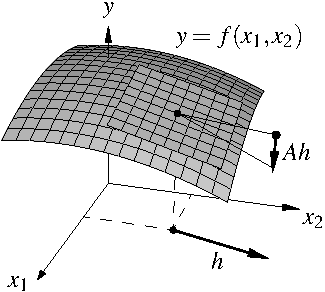
\includegraphics{figures/svder}
\caption{Illustration of a derivative for a function $f \colon \R^2 \to \R$.  The vector $h$ is shown
in the $x_1x_2$-plane based at $(x_1,x_2)$, and the vector
$Ah \in \R^1$ is shown along the $y$ direction.\label{fig:svder}}
\end{myfigureht}

For a differentiable function,
the derivative of $f$ is a function from $U$ to $L(\R^n,\R^m)$.  Compare
to the one dimensional case, where the derivative is a function
from $U$ to $\R$, but we really want to think of $\R$ here as
$L(\R^1,\R^1)$.  As in one dimension, the idea is that a differentiable
mappings is ``infinitesimally close'' to a linear mappings, and this
linear mapping is the derivative.

The norms above must be on the right spaces of course.  The norm in the
numerator is on $\R^m$, and the norm in the denominator is on $\R^n$ where $h$
lives.
Normally it is 
understood that $h \in \R^n$ from context.
We will not explicitly say so from now on.

We have again cheated somewhat and said that $A$
is \emph{the} derivative.  We have not shown yet that there
is only one, let us do that now.

\begin{prop}
Let $U \subset \R^n$ be an open subset and $f \colon U \to \R^m$.  Suppose
$x \in U$ and there exist 
$A,B \in L(\R^n,\R^m)$ such that
\begin{equation*}
\lim_{h \to 0}
\frac{\snorm{f(x+h)-f(x) - Ah}}{\snorm{h}} = 0
\qquad \text{and} \qquad
\lim_{h \to 0}
\frac{\snorm{f(x+h)-f(x) - Bh}}{\snorm{h}} = 0 .
\end{equation*}
Then $A=B$.
\end{prop}

\begin{proof}
\begin{equation*}
\begin{split}
\frac{\snorm{(A-B)h}}{\snorm{h}} & =
\frac{\snorm{f(x+h)-f(x) - Ah - (f(x+h)-f(x) - Bh)}}{\snorm{h}} \\
& \leq
\frac{\snorm{f(x+h)-f(x) - Ah}}{\snorm{h}} + \frac{\snorm{f(x+h)-f(x) -
Bh}}{\snorm{h}} .
\end{split}
\end{equation*}
So 
$\frac{\snorm{(A-B)h}}{\snorm{h}} \to 0$ as $h \to 0$.  That is, given
$\epsilon > 0$, then for all $h$ in some $\delta$-ball around
the origin
\begin{equation*}
\epsilon > 
\frac{\snorm{(A-B)h}}{\snorm{h}}
=
\norm{(A-B)\frac{h}{\snorm{h}}} .
\end{equation*}
%But $\frac{h}{\snorm{h}}$ is of norm 1.  
For any $x$ with $\snorm{x}=1$,
let $h = (\nicefrac{\delta}{2}) \, x$, then $\snorm{h} < \delta$
and $\frac{h}{\snorm{h}} = x$.
So $\snorm{(A-B)x} < \epsilon$.  Taking the supremum over all $x$ with
$\snorm{x} = 1$ we get the operator norm
$\snorm{A-B} \leq \epsilon$.  As $\epsilon > 0$
was arbitrary $\snorm{A-B} = 0$ or in other words $A = B$.
\end{proof}

\begin{example}
If $f(x) = Ax$ for a linear mapping $A$, then
$f'(x) = A$.  This is easily seen:
\begin{equation*}
\frac{\snorm{f(x+h)-f(x) - Ah}}{\snorm{h}}
=
\frac{\snorm{A(x+h)-Ax - Ah}}{\snorm{h}}
=
\frac{0}{\snorm{h}} = 0 .
\end{equation*}
\end{example}

\begin{example}
Let $f \colon \R^2 \to \R^2$ be defined by
\begin{equation*}
f(x,y) = \bigl(f_1(x,y),f_2(x,y)\bigr) := (1+x+2y+x^2,2x+3y+xy).
\end{equation*}
Let us show that $f$ is differentiable at the origin and let us 
compute the derivative,
directly using the definition.  The derivative is in $L(\R^2,\R^2)$ so it can be
represented by a $2\times 2$ matrix
$\left[\begin{smallmatrix}a&b\\c&d\end{smallmatrix}\right]$.  Suppose $h =
(h_1,h_2)$.  We need the following expression to go to zero.
\begin{multline*}
\frac{\snorm{
f(h_1,h_2)-f(0,0)
-
(ah_1 +bh_2 , ch_1+dh_2)}
}{\snorm{(h_1,h_2)}}
=
\\
\frac{\sqrt{
{\bigl((1-a)h_1 + (2-b)h_2 + h_1^2\bigr)}^2
+
{\bigl((2-c)h_1 + (3-d)h_2 + h_1h_2\bigr)}^2}}{\sqrt{h_1^2+h_2^2}} .
\end{multline*}
If we choose $a=1$, $b=2$, $c=2$, $d=3$, the expression becomes
\begin{equation*}
\frac{\sqrt{
h_1^4 + h_1^2h_2^2}}{\sqrt{h_1^2+h_2^2}}
=
\abs{h_1}
\frac{\sqrt{
h_1^2 + h_2^2}}{\sqrt{h_1^2+h_2^2}}
= \abs{h_1} .
\end{equation*}
And this expression does indeed go to zero as $h \to 0$.  Therefore the
function is differentiable at the origin and 
the derivative can be represented by the matrix
$\left[\begin{smallmatrix}1&2\\2&3\end{smallmatrix}\right]$.
\end{example}

\begin{prop}
Let $U \subset \R^n$ be open and $f \colon U \to \R^m$ be
differentiable at $p \in U$.  Then $f$ is continuous at $p$.
\end{prop}

\begin{proof}
Another way to write the differentiability of $f$ at $p$ is to first write
\begin{equation*}
r(h) := f(p+h)-f(p) - f'(p) h ,
\end{equation*}
and $\frac{\snorm{r(h)}}{\snorm{h}}$ must go to zero as $h \to 0$.
So
$r(h)$ itself must go to zero.  The mapping $h \mapsto f'(p) h$
is a linear mapping between finite dimensional spaces, it is
therefore continuous
and goes to zero as $h \to 0$.  Therefore,
$f(p+h)$ must go to $f(p)$ as $h \to 0$.  That is, $f$ is continuous at $p$.
\end{proof}

If $A \in L(X,Y)$ and $B \in L(Y,Z)$ are linear maps, then we
saw that they are their own derivative.  The composition
$BA \in L(X,Z)$ is therefore also its own derivative, and
so the derivative of the composition is the composition
of the derivatives.  As differentiable maps are ``infinitesimally close''
to linear maps, they have the same property:

%\textbf{Theorem 9.15 (Chain rule):}
\begin{thm}[Chain rule]
Let $U \subset \R^n$ be open and let $f \colon U \to \R^m$ be
differentiable at $p \in U$.  Let $V \subset \R^m$ be open,
$f(U) \subset V$ and let $g \colon V \to \R^\ell$ be differentiable
at $f(p)$.  Then
\begin{equation*}
F(x) = g\bigl(f(x)\bigr)
\end{equation*}
is differentiable at $p$ and
\begin{equation*}
F'(p) = g'\bigl(f(p)\bigr) f'(p) .
\end{equation*}
\end{thm}

Without the points where things are evaluated, this is sometimes written as
$F' = {(f \circ g)}' = g' f'$.  The way to
understand it is that the derivative of the composition $g \circ f$
is the composition of the derivatives of $g$ and $f$.  That is, if
$f'(p) = A$ and $g'\bigl(f(p)\bigr) = B$, then $F'(p) = BA$,
just as it is for linear maps.

\begin{proof}
Let $A := f'(p)$ and $B := g'\bigl(f(p)\bigr)$.  Take $h \in \R^n$
and write $q = f(p)$, $k = f(p+h)-f(p)$.  Let
\begin{equation*}
r(h) := f(p+h)-f(p) - A h . %= k - Ah.
\end{equation*}
Then $r(h) = k-Ah$ or $Ah = k-r(h)$.  We look at the quantity we need to go
to zero:
\begin{equation*}
\begin{split}
\frac{\snorm{F(p+h)-F(p) - BAh}}{\snorm{h}}
& =
\frac{\snorm{g\bigl(f(p+h)\bigr)-g\bigl(f(p)\bigr) - BAh}}{\snorm{h}}
\\
& =
\frac{\snorm{g(q+k)-g(q) - B\bigl(k-r(h)\bigr)}}{\snorm{h}}
\\
%& =
%\frac
%{\snorm{g(q+k)-g(q) - B\bigl(k-r(h)\bigr)}}
%{\snorm{k}}
%\frac
%{\snorm{f(p+h)-f(p)}}
%{\snorm{h}}
%\\
& \leq
\frac
{\snorm{g(q+k)-g(q) - Bk}}
{\snorm{h}}
+
\snorm{B}
\frac
{\snorm{r(h)}}
{\snorm{h}}
\\
& =
\frac
{\snorm{g(q+k)-g(q) - Bk}}
{\snorm{k}}
\frac
{\snorm{f(p+h)-f(p)}}
{\snorm{h}}
+
\snorm{B}
\frac
{\snorm{r(h)}}
{\snorm{h}} .
\end{split}
\end{equation*}
First, $\snorm{B}$ is constant and $f$ is differentiable at $p$,
so
the term $\snorm{B}\frac{\snorm{r(h)}}{\snorm{h}}$ goes to 0.
Next as $f$ is continuous at $p$, we have that as 
$h$ goes to 0, then $k$ goes to 0.  Therefore
$\frac
{\snorm{g(q+k)-g(q) - Bk}}
{\snorm{k}}$ goes to 0 because $g$ is differentiable at $q$.
Finally 
\begin{equation*}
\frac
{\snorm{f(p+h)-f(p)}}
{\snorm{h}}
\leq
\frac
{\snorm{f(p+h)-f(p)-Ah}}
{\snorm{h}}
+
\frac
{\snorm{Ah}}
{\snorm{h}}
\leq
\frac
{\snorm{f(p+h)-f(p)-Ah}}
{\snorm{h}}
+
\snorm{A} .
\end{equation*}
As $f$ is differentiable at $p$,
for small enough $h$
${\snorm{f(p+h)-f(p)-Ah}}
{\snorm{h}}$ is bounded.  Therefore the
term
$
\frac
{\snorm{f(p+h)-f(p)}}
{\snorm{h}}
$
stays bounded as $h$ goes to 0.  Therefore, 
$\frac{\snorm{F(p+h)-F(p) - BAh}}{\snorm{h}}$ goes to zero, and
$F'(p) = BA$, which is what was claimed.
\end{proof}

\subsection{Partial derivatives}

There is another way to generalize the derivative from one dimension.
We hold all but one variable constant and take the regular
derivative.

\begin{defn}
Let
$f \colon U \to \R$ be a function on an open set $U \subset \R^n$.
If the following limit exists we write
\glsadd{not:partialder}
\begin{equation*}
\frac{\partial f}{\partial x_j} (x) := 
\lim_{h\to 0}\frac{f(x_1,\ldots,x_{j-1},x_j+h,x_{j+1},\ldots,x_n)-f(x)}{h}
=
\lim_{h\to 0}\frac{f(x+h e_j)-f(x)}{h} .
\end{equation*}
We call 
$\frac{\partial f}{\partial x_j} (x)$ the \emph{\myindex{partial derivative}}
of $f$
with respect to $x_j$.  Sometimes we write $D_j f$ instead.
See \figureref{fig:svpartder}.

For a mapping $f \colon U \to \R^m$ we write
$f = (f_1,f_2,\ldots,f_m)$, where $f_k$ are real-valued
functions.  We then take partial derivatives of
the components,
$\frac{\partial f_k}{\partial x_j}$ (or write it as $D_j f_k$).
\end{defn}

\begin{myfigureht}
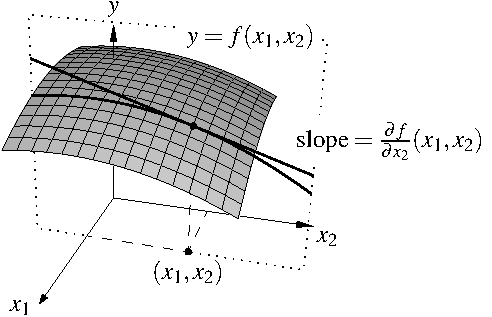
\includegraphics{figures/svpartder}
\caption{Illustration of a partial derivative for a function $f \colon \R^2
\to \R$.  The slope of the given line in the $yx_2$-plane is
$\frac{\partial f}{\partial x_2}(x_1,x_2)$.\label{fig:svpartder}}
\end{myfigureht}

Partial derivatives are easier to compute with all the machinery of
calculus, and they provide a way to compute the derivative of a
function.

%\textbf{Theorem 9.17:}
\begin{prop} \label{mv:prop:jacobianmatrix}
Let $U \subset \R^n$ be open and let $f \colon U \to \R^m$ be
differentiable at $p \in U$.  Then all the partial derivatives at $p$
exist and in terms of the standard basis of $\R^n$ and $\R^m$,
$f'(p)$ is represented by the matrix
\begin{equation*}
\begin{bmatrix}
\frac{\partial f_1}{\partial x_1}(p)
&
\frac{\partial f_1}{\partial x_2}(p)
& \ldots &
\frac{\partial f_1}{\partial x_n}(p)
\\
\frac{\partial f_2}{\partial x_1}(p)
&
\frac{\partial f_2}{\partial x_2}(p)
& \ldots &
\frac{\partial f_2}{\partial x_n}(p)
\\
\vdots & \vdots & \ddots & \vdots
\\
\frac{\partial f_m}{\partial x_1}(p)
&
\frac{\partial f_m}{\partial x_2}(p)
& \ldots &
\frac{\partial f_m}{\partial x_n}(p)
\end{bmatrix} .
\end{equation*}
\end{prop}


In other words
\begin{equation*}
f'(p) \, e_j =
\sum_{k=1}^m
\frac{\partial f_k}{\partial x_j}(p) \,e_k .
\end{equation*}
If $v = \sum_{j=1}^n c_j e_j = (c_1,c_2,\ldots,c_n)$, then
\begin{equation*}
f'(p) \, v =
\sum_{j=1}^n
\sum_{k=1}^m
 c_j
\frac{\partial f_k}{\partial x_j}(p) \,e_k
=
\sum_{k=1}^m
\left(
\sum_{j=1}^n
 c_j
\frac{\partial f_k}{\partial x_j}(p) \right) \,e_k .
\end{equation*}

\begin{proof}
Fix a $j$ and note that
\begin{equation*}
\begin{split}
\norm{\frac{f(p+h e_j)-f(p)}{h} - f'(p) e_j} & = 
\norm{\frac{f(p+h e_j)-f(p) - f'(p) h e_j}{h}} \\
& =
\frac{\snorm{f(p+h e_j)-f(p) - f'(p) h e_j}}{\snorm{h e_j}} .
\end{split}
\end{equation*}
As $h$ goes to 0, the right hand side goes to zero by
differentiability of $f$, and hence
\begin{equation*}
\lim_{h \to 0}
\frac{f(p+h e_j)-f(p)}{h} = f'(p) e_j  .
\end{equation*}
Note that $f$ is vector valued.  So represent $f$ by components
$f = (f_1,f_2,\ldots,f_m)$, and note that taking a limit in $\R^m$
is the same as taking the limit in each component separately.  Therefore
for any $k$
the partial derivative
\begin{equation*}
\frac{\partial f_k}{\partial x_j} (p)
=
\lim_{h \to 0}
\frac{f_k(p+h e_j)-f_k(p)}{h}
\end{equation*}
exists and 
is equal to the $k$th component of $f'(p) e_j$, and we are done.
\end{proof}

The converse of the proposition is not true.  Just because the partial
derivatives exist, does not mean that the function is differentiable.  See
the exercises.
However, when the partial derivatives are continuous, we will prove that the
converse holds.
One of the consequences of the proposition is that if $f$
is differentiable on $U$, then $f' \colon U \to
L(\R^n,\R^m)$ is a continuous function if and only if
all the $\frac{\partial f_k}{\partial x_j}$ are continuous functions.

\subsection{Gradient and directional derivatives}

Let $U \subset \R^n$ be open and $f \colon U \to \R$ is a differentiable
function.  We define
the \emph{\myindex{gradient}} as
\glsadd{not:gradient}
\begin{equation*}
\nabla f (x) := \sum_{j=1}^n \frac{\partial f}{\partial x_j} (x)\, e_j .
\end{equation*}
The gradient gives a way to represent the action of
the derivative as a dot product: $f'(x)v = \nabla f(x) \cdot v$.

Suppose $\gamma \colon (a,b) \subset \R \to \R^n$ is a differentiable
function and the image $\gamma\bigl((a,b)\bigr) \subset U$.
Such a function and its image is sometimes called a \emph{\myindex{curve}},
or a \emph{\myindex{differentiable curve}}.
Write $\gamma =
(\gamma_1,\gamma_2,\ldots,\gamma_n)$.  Let
\begin{equation*}
g(t) := f\bigl(\gamma(t)\bigr) .
\end{equation*}
The function
$g$ is differentiable.  For purposes of computation we 
identify $L(\R^1)$ with $\R$, and hence $g'(t)$ can be computed as
a number:
\begin{equation*}
g'(t) =
f'\bigl(\gamma(t)\bigr) \gamma^{\:\prime}(t)
=
\sum_{j=1}^n
\frac{\partial f}{\partial x_j} \bigl(\gamma(t)\bigr)
\frac{d\gamma_j}{dt} (t)
=
\sum_{j=1}^n
\frac{\partial f}{\partial x_j}
\frac{d\gamma_j}{dt} .
\end{equation*}
For convenience,
we sometimes 
leave out the points where we are evaluating as on the right hand side above.
Let us rewrite this with the notation of the gradient and the dot product:
\begin{equation*}
g'(t) = (\nabla f) \bigl(\gamma(t)\bigr) \cdot \gamma^{\:\prime}(t)
= \nabla f \cdot \gamma^{\:\prime} .
\end{equation*}

We use this idea to define derivatives in a specific direction.  A direction
is simply a vector pointing in that direction.  So pick a vector $u \in \R^n$
such that $\snorm{u} = 1$, and fix $x \in U$.
Then define the curve
\begin{equation*}
\gamma(t) := x + tu .
\end{equation*}
Then $\gamma^{\:\prime}(t) = u$ for all $t$.  
By the chain rule
\begin{equation*}
\frac{d}{dt}\Big|_{t=0} \bigl[ f(x+tu) \bigr] =
(\nabla f) (x) \cdot u ,
\end{equation*}
where the notation
$\frac{d}{dt}\big|_{t=0}$ represents the derivative evaluated at $t=0$.
We also compute directly
\begin{equation*}
\frac{d}{dt}\Big|_{t=0} \bigl[ f(x+tu) \bigr] =
\lim_{h\to 0}
\frac{f(x+hu)-f(x)}{h} .
\end{equation*}
We obtain the \emph{\myindex{directional derivative}},
denoted by
\glsadd{not:mvdirder}
\begin{equation*}
D_u f (x) := \frac{d}{dt}\Big|_{t=0} \bigl[ f(x+tu) \bigr] ,
\end{equation*}
which can be computed by one of the methods above.

Let us suppose $(\nabla f)(x) \neq 0$.
By Cauchy--Schwarz inequality we have
\begin{equation*}
\abs{D_u f(x)} \leq \snorm{(\nabla f)(x)} .
\end{equation*}
Equality is achieved when $u$ is a scalar multiple of
$(\nabla f)(x)$.  That is, when
\begin{equation*}
u = 
\frac{(\nabla f)(x)}{\snorm{(\nabla f)(x)}} ,
\end{equation*}
we get $D_u f(x) = \snorm{(\nabla f)(x)}$.
The gradient points in the direction in which the
function grows fastest, in other words, in the direction in which $D_u f(x)$ is maximal.

\subsection{The Jacobian}

\begin{defn}
Let $U \subset \R^n$ and
$f \colon U \to \R^n$ be a differentiable mapping.  Then define the
\emph{\myindex{Jacobian}}, or 
\emph{\myindex{Jacobian determinant}}%
\footnote{The matrix from \propref{mv:prop:jacobianmatrix} representing $f'(x)$
is sometimes called the
\emph{\myindex{Jacobian matrix}}.},
of $f$ at $x$ as
\glsadd{not:jacobdet}
\begin{equation*}
J_f(x) := \det\bigl( f'(x) \bigr) .
\end{equation*}
Sometimes this is written as
\begin{equation*}
\frac{\partial(f_1,f_2,\ldots,f_n)}{\partial(x_1,x_2,\ldots,x_n)} .
\end{equation*}
\end{defn}

This last piece of notation may seem somewhat confusing,
but it is useful when you need to specify
the exact variables and function components used.

The Jacobian $J_f$ is a real valued function, and when $n=1$ it is simply the
derivative.
%When $f$ is $C^1$, then $J_f$ is a continuous function.
From the chain rule and the fact that $\det(AB) = \det(A)\det(B)$, it follows that:
\begin{equation*}
J_{f \circ g} (x) = J_f\bigl(g(x)\bigr) J_g(x) .
\end{equation*}

The determinant of a linear mapping tells us what happens to
area/volume under the mapping.
Similarly, the Jacobian measures how much a differentiable mapping stretches
things locally, and if it flips orientation.  In particular, if the Jacobian
is non-zero than we would assume that locally the mapping is invertible (and
we would be correct as we will later see).

\subsection{Exercises}

\begin{exercise}
Suppose $\gamma \colon (-1,1) \to \R^n$ and
$\alpha \colon (-1,1) \to \R^n$ be two differentiable curves
such that $\gamma(0) = \alpha(0)$ and $\gamma^{\:\prime}(0) = \alpha'(0)$.
Suppose $F \colon \R^n \to \R$ is a differentiable function.  Show that
\begin{equation*}
\frac{d}{dt}\Big|_{t=0}
F\bigl(\gamma(t)\bigr)
=
\frac{d}{dt}\Big|_{t=0}
F\bigl(\alpha(t)\bigr)
.
\end{equation*}
\end{exercise}

\begin{exercise}
Let $f \colon \R^2 \to \R$ be given by
%\begin{equation}
$f(x,y)
=
\sqrt{x^2+y^2}$.
%\end{equation}
Show that $f$ is not differentiable at the origin.
See \figureref{fig:distfromorgfunc}.
\end{exercise}

\begin{myfigureht}
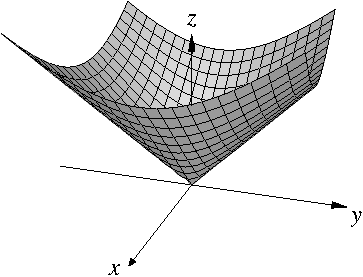
\includegraphics{figures/distfromorgfunc}
\caption{Graph of $\sqrt{x^2+y^2}$.\label{fig:distfromorgfunc}}
\end{myfigureht}

\begin{exercise}
Using only the definition of the derivative, show that
the following $f \colon \R^2 \to \R^2$ are differentiable at the origin and
find their derivative.
\\
a) $f(x,y) := (1+x+xy,x)$,
\\
b) $f(x,y) := (y-y^{10},x)$,
\\
c) $f(x,y) := \bigl( (x+y+1)^2 , (x-y+2)^2 \bigr)$.
\end{exercise}

\begin{exercise}
Suppose $f \colon \R \to \R$ and $g \colon \R \to \R$ are differentiable
functions.  Using only the definition of the derivative, show that
$h \colon \R^2 \to \R^2$ defined by $h(x,y)
:= \bigl(f(x),g(y)\bigr)$ is a differentiable function and find the
derivative at any point $(x,y)$.
\end{exercise}

\begin{exercise} \label{exercise:noncontpartialsexist}
Define a function $f \colon \R^2 \to \R$ by
\begin{equation*}
f(x,y)
:=
\begin{cases}
\frac{xy}{x^2+y^2} & \text{ if $(x,y) \not= (0,0)$}, \\
0 & \text{ if $(x,y) = (0,0)$}.
\end{cases}
\end{equation*}
See \figureref{fig:xyxsqysqvol2}.\\
a)~Show that partial derivatives 
$\frac{\partial f}{\partial x}$ and
$\frac{\partial f}{\partial y}$ exist at all points (including the origin).\\
b)~Show that $f$ is not continuous at the origin (and hence not
differentiable).
\end{exercise}

\begin{myfigureht}
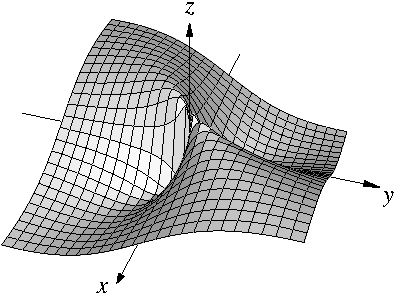
\includegraphics{figures/xyxsqysq}
\caption{Graph of $\frac{xy}{x^2+y^2}$.\label{fig:xyxsqysqvol2}}
\end{myfigureht}

\begin{samepage}
\begin{exercise}
Define a function $f \colon \R^2 \to \R$ by
\begin{equation*}
f(x,y)
:=
\begin{cases}
\frac{x^2y}{x^2+y^2} & \text{ if $(x,y) \not= (0,0)$}, \\
0 & \text{ if $(x,y) = (0,0)$}.
\end{cases}
\end{equation*}
See \figureref{fig:xsqyxsqysq}.\\
a)~Show that partial derivatives 
$\frac{\partial f}{\partial x}$ and
$\frac{\partial f}{\partial y}$ exist at all points.\\
b)~Show that for all $u \in \R^2$ with $\snorm{u}=1$, the directional
derivative $D_u f$ exists at all points.\\
c)~Show that $f$ is continuous at the origin.\\
d)~Show that $f$ is not differentiable at the origin.
\end{exercise}
\end{samepage}

\begin{myfigureht}
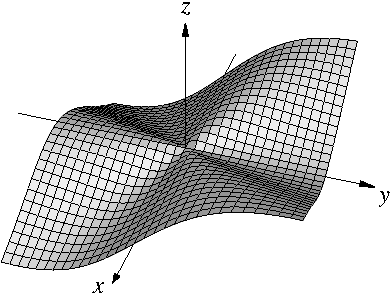
\includegraphics{figures/xsqyxsqysq}
\caption{Graph of $\frac{x^2y}{x^2+y^2}$.\label{fig:xsqyxsqysq}}
\end{myfigureht}

\begin{exercise}
Suppose $f \colon \R^n \to \R^n$ is one-to-one, onto, differentiable at all
points, and such that $f^{-1}$ is also differentiable at all points.\\
a) Show that $f'(p)$ is invertible at all points $p$ and compute
${(f^{-1})}'\bigl(f(p)\bigr)$.  Hint: consider $p = f^{-1}\bigl(f(p)\bigr)$.\\
b) Let $g \colon \R^n \to \R^n$ be a function differentiable at $q \in \R^n$
and such that $g(q)=q$.  Suppose $f(p) = q$ for some $p \in \R^n$.
Show $J_g(q) = J_{f^{-1} \circ g \circ f}(p)$ where $J_g$ is the Jacobian
determinant.
\end{exercise}

\begin{exercise}
Suppose $f \colon \R^2 \to \R$ is differentiable and such that
$f(x,y) = 0$ if and only if $y=0$ and such that $\nabla f(0,0) = (1,1)$.
Prove that $f(x,y) > 0$ whenever $y > 0$, and
$f(x,y) < 0$ whenever $y < 0$.
\end{exercise}

\begin{exercise} \label{exercise:mv:maximumcritical}
Suppose $U \subset \R^n$ is open and
$f \colon U \to \R$ is differentiable.  Suppose $f$ has a local maximum
at $p \in U$.  Show that $f'(p) = 0$, that is the zero mapping in
$L(\R^n,\R)$.  That is $p$ is a
\emph{\myindex{critical point}} of $f$.
\end{exercise}

\begin{exercise}
Suppose $f \colon \R^2 \to \R$ is differentiable and suppose that
whenever $x^2+y^2 = 1$, then $f(x,y) = 0$.  Prove that there exists at least
one point $(x_0,y_0)$ such that
$\frac{\partial f}{\partial x}(x_0,y_0) = \frac{\partial f}{\partial
y}(x_0,y_0) = 0$.
\end{exercise}

\begin{exercise}[The \myindex{Peano surface}]
Define $f(x,y) := ( x-y^2 ) ( 2 y^2 - x)$.  Show\\
a) $(0,0)$ is a critical point, that is $f'(0,0) = 0$, that is the zero
linear map in $L(\R^2,\R)$.\\
b) For every direction, that is $(x,y)$ such that $x^2+y^2=1$ the
``restriction of $f$ to the line containing the points $(0,0)$ and
$(x,y)$'', that is a function $g(t) := f(tx,ty)$ has a local maximum at
$t=0$.\\
c) $f$ does not have a local maximum at $(0,0)$.
\end{exercise}

\begin{exercise}
Suppose $f \colon \R \to \R^n$ is differentiable and $\snorm{f(t)} = 1$ for
all $t$ (that is, we have a curve in the unit sphere).  Then show that for
all $t$, treating $f'$ as a vector we have, $f'(t) \cdot f(t) = 0$.
\end{exercise}

\begin{exercise}
Define $f \colon \R^2 \to \R^2$ by $f(x,y) :=
\bigl(x,y+\varphi(x)\bigr)$ for some differentiable function $\varphi$ of one
variable.  Show $f$ is differentiable and find $f'$.
\end{exercise}

%%%%%%%%%%%%%%%%%%%%%%%%%%%%%%%%%%%%%%%%%%%%%%%%%%%%%%%%%%%%%%%%%%%%%%%%%%%%%%

\sectionnewpage
\section{Continuity and the derivative}
\label{sec:svthedercont}

\sectionnotes{1--2 lectures}

\subsection{Bounding the derivative}

Let us prove a ``mean value theorem'' for vector valued functions.

%\textbf{Theorem 5.19:}
\begin{lemma}
If $\varphi \colon [a,b] \to \R^n$ is differentiable on $(a,b)$ and
continuous on $[a,b]$, then there exists a $t_0 \in (a,b)$ such that
\begin{equation*}
\snorm{\varphi(b)-\varphi(a)} \leq (b-a) \snorm{\varphi'(t_0)} .
\end{equation*}
\end{lemma}

\begin{proof}
By mean value theorem on the function
$\bigl(\varphi(b)-\varphi(a) \bigr) \cdot \varphi(t)$
(the dot is the scalar dot product again) we obtain
there is a $t_0 \in (a,b)$ such that
\begin{equation*}
\bigl(\varphi(b)-\varphi(a) \bigr) \cdot \varphi(b) - 
\bigl(\varphi(b)-\varphi(a) \bigr) \cdot \varphi(a)  = 
\snorm{\varphi(b)-\varphi(a)}^2
=
(b-a)
\bigl(\varphi(b)-\varphi(a) \bigr) \cdot \varphi'(t_0)
\end{equation*}
where we treat $\varphi'$ as a simply a column vector of numbers by abuse of
notation.  Note that
in this case, if we think of $\varphi'(t)$ as simply a vector, then by
\exerciseref{exercise:normonedim},
$\snorm{\varphi'(t)}_{L(\R,\R^n)} = \snorm{\varphi'(t)}_{\R^n}$.
That is, the euclidean norm of the vector is the same as the operator norm
of $\varphi'(t)$.

By Cauchy--Schwarz inequality
\begin{equation*}
\snorm{\varphi(b)-\varphi(a)}^2
=
(b-a)\bigl(\varphi(b)-\varphi(a) \bigr) \cdot \varphi'(t_0)
\leq
(b-a)
\snorm{\varphi(b)-\varphi(a)} \snorm{\varphi'(t_0)} . \qedhere
\end{equation*}
\end{proof}

Recall that a set $U$ is convex
if whenever $x,y \in U$, the line segment from
$x$ to $y$ lies in $U$.

\begin{prop} \label{mv:prop:convexlip}
%\textbf{Theorem 9.19:}
Let $U \subset \R^n$ be a convex open set, $f \colon U \to \R^m$
a differentiable function, and an $M$ such that
\begin{equation*}
\snorm{f'(x)} \leq M
\end{equation*}
for all $x \in U$.  Then $f$ is Lipschitz with constant $M$, that is
\begin{equation*}
\snorm{f(x)-f(y)} \leq M \snorm{x-y}
\end{equation*}
for all $x,y \in U$.
\end{prop}

\begin{proof}
Fix $x$ and $y$ in $U$ and note that
$(1-t)x+ty \in U$ for all $t \in [0,1]$
by convexity.
Next
\begin{equation*}
\frac{d}{dt} \Bigl[f\bigl((1-t)x+ty\bigr)\Bigr]
=
f'\bigl((1-t)x+ty\bigr) (y-x) .
\end{equation*}
By the mean value theorem above we get for
some $t_0 \in (0,1)$
\begin{equation*}
\snorm{f(x)-f(y)} \leq
\norm{\frac{d}{dt} \Big|_{t=t_0} \Bigl[ f\bigl((1-t)x+ty\bigr) \Bigr] } \leq
\snorm{f'\bigl((1-t_0)x+t_0y\bigr)} \snorm{y-x} \leq
M \snorm{y-x} . \qedhere
\end{equation*}
\end{proof}

\begin{example}
If $U$ is not convex the proposition is not true.  To see this fact, take
the set
\begin{equation*}
U = \{ (x,y) : 0.5 < x^2+y^2 < 2 \} \setminus \{ (x,0) : x < 0 \} .
\end{equation*}
Let $f(x,y)$ be the angle that the line from the origin to $(x,y)$
makes with the positive $x$ axis.  You can even write the formula for $f$:
\begin{equation*}
f(x,y) = 2 \operatorname{arctan}\left( \frac{y}{x+\sqrt{x^2+y^2}}\right) .
\end{equation*}
Think spiral staircase with room in the middle.  See
\figureref{mv:fignonlip}.

\begin{myfigureht}
\subimport*{figures/}{example-nonlip.pdf_t}
\qquad
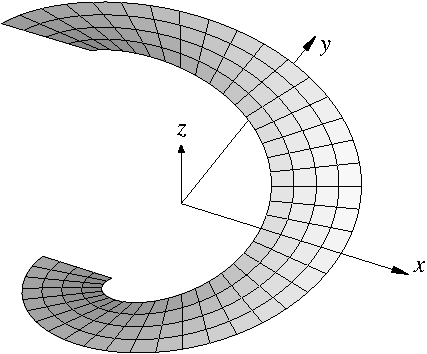
\includegraphics{figures/nonlipgraph}
\caption{A non-Lipschitz function with uniformly bounded
derivative.\label{mv:fignonlip}}
\end{myfigureht}

The function is differentiable,
and the derivative is bounded on $U$, which is not hard to see.   Think of
what happens near where the negative $x$-axis cuts the annulus in half.
As we approach this cut from top (positive $y$), $f(x,y)$ approaches $\pi$.
From the bottom (from negative $y$), $f(x,y)$ approaches $-\pi$.
So for small $\epsilon > 0$, $\abs{f(-1,\epsilon)-f(-1,-\epsilon)}$
approaches $2\pi$, but $\snorm{(-1,\epsilon)-(-1,-\epsilon)} = 2\epsilon$,
which is arbitrarily small.  The conclusion of the proposition does not
hold for this nonconvex $U$.
%To see that the derivative is
%bounded, we note that it is not hard to see that the derivative will not
%depend on the rotation, so we can just do it at $y=0$, and we 
\end{example}

Let us solve the differential equation $f' = 0$.

\begin{cor}
If $U \subset \R^n$ is connected and $f \colon U \to \R^m$ is differentiable
and $f'(x) = 0$, for all $x \in U$, then $f$ is constant.
\end{cor}

\begin{proof}
For any $x \in U$, there is a ball $B(x,\delta) \subset U$.  The ball
$B(x,\delta)$ is convex.  Since
$\snorm{f'(y)} \leq 0$ for all $y \in B(x,\delta)$, then by the theorem,
$\snorm{f(x)-f(y)} \leq 0 \snorm{x-y} = 0$.  So $f(x) = f(y)$ for all $y \in
B(x,\delta)$.

This means that $f^{-1}(c)$ is open for any $c \in \R^m$.  Suppose
$f^{-1}(c)$ is nonempty.  
The two sets
\begin{equation*}
U' = f^{-1}(c), \qquad U'' = f^{-1}(\R^m\setminus\{c\}) =
\bigcup_{\substack{a \in \R^m\\a\neq c}} f^{-1}(a)
\end{equation*}
are open disjoint, and further $U = U' \cup U''$.  So as $U'$ is nonempty,
and $U$ is connected,
we have that $U'' = \emptyset$.  So $f(x) = c$ for all $x \in U$.
\end{proof}

\subsection{Continuously differentiable functions}

\begin{defn}
Let $U \subset \R^n$ be open.
We say $f \colon U \to \R^m$ is
\emph{\myindex{continuously differentiable}},
or $C^1(U)$\glsadd{not:C1},
if $f$ is differentiable and $f' \colon U \to L(\R^n,\R^m)$
is continuous.
\end{defn}

%\textbf{Theorem 9.21:}
\begin{prop} \label{mv:prop:contdiffpartials}
Let $U \subset \R^n$ be open and
$f \colon U \to \R^m$.  The function
$f$ is continuously differentiable if and only if all
the partial derivatives exist and are continuous.
\end{prop}

Without continuity the theorem does not hold.  Just because
partial derivatives exist does not mean that $f$ is differentiable,
in fact, $f$ may not even be continuous.  See the exercises
for the last section and also for this section.

\begin{proof}
We have seen that if $f$ is differentiable, then
the partial derivatives exist.  Furthermore, the partial
derivatives are the entries of the matrix of $f'(x)$.  So if
$f' \colon U \to L(\R^n,\R^m)$ is continuous, then the entries are
continuous, hence the partial derivatives are continuous.

To prove the opposite direction,
suppose the partial derivatives exist and are continuous.
Fix $x \in U$.  If we show that $f'(x)$ exists we are done, because
the entries of the matrix $f'(x)$ are then the partial derivatives and if
the entries are continuous functions, the matrix valued function $f'$ is
continuous.

Let us do induction on dimension.  First let us note that
the conclusion is true when $n=1$.  In this case the derivative
is just the regular derivative (exercise: you should check that the fact
that the function is vector valued is not a problem).

Suppose the conclusion is true for $\R^{n-1}$,
that is,
if we restrict to the first $n-1$ variables, the conclusion is true.
It is easy to see that the first $n-1$
partial derivatives of $f$ restricted to the set where the last coordinate is
fixed are the same as those for $f$.
In the following
we think of $\R^{n-1}$ as a subset of $\R^n$, that is the set in $\R^n$ where $x_n = 0$.
Let
\begin{equation*}
A = 
\begin{bmatrix}
\frac{\partial f_1}{\partial x_1}(x)
& \ldots &
\frac{\partial f_1}{\partial x_n}(x)
\\
\vdots & \ddots & \vdots
\\
\frac{\partial f_m}{\partial x_1}(x)
& \ldots &
\frac{\partial f_m}{\partial x_n}(x)
\end{bmatrix} ,
\qquad
A_1 = 
\begin{bmatrix}
\frac{\partial f_1}{\partial x_1}(x)
& \ldots &
\frac{\partial f_1}{\partial x_{n-1}}(x)
\\
\vdots & \ddots & \vdots
\\
\frac{\partial f_m}{\partial x_1}(x)
& \ldots &
\frac{\partial f_m}{\partial x_{n-1}}(x)
\end{bmatrix} ,
\qquad
v = 
%\frac{\partial f}{\partial x_n}(x) =
\begin{bmatrix}
\frac{\partial f_1}{\partial x_n}(x)
\\
\vdots
\\
\frac{\partial f_m}{\partial x_n}(x)
\end{bmatrix} .
\end{equation*}
Let $\epsilon > 0$ be given.  Let $\delta > 0$ be such that
for any $k \in \R^{n-1}$ with $\snorm{k} < \delta$ we have
\begin{equation*}
\frac{\snorm{f(x+k) - f(x) - A_1k}}{\snorm{k}} < \epsilon .
\end{equation*}
By continuity of the partial derivatives, suppose $\delta$ is small
enough so that
\begin{equation*}
\abs{\frac{\partial f_j}{\partial x_n}(x+h)
      - \frac{\partial f_j}{\partial x_n}(x)} < \epsilon ,
\end{equation*}
for all $j$ and all $h$ with $\snorm{h} < \delta$.

Let $h = h_1 + t e_n$ be a vector in $\R^n$ where $h_1 \in \R^{n-1}$ such that
$\snorm{h} < \delta$.  Then $\snorm{h_1} \leq \snorm{h} < \delta$.
Note that $Ah = A_1h_1 + tv$.
\begin{equation*}
\begin{split}
\snorm{f(x+h) - f(x) - Ah}
& = \snorm{f(x+h_1 + t e_n) - f(x+h_1) - tv + f(x+h_1) - f(x) - A_1h_1}
\\
& \leq \snorm{f(x+h_1 + t e_n) - f(x+h_1) -tv} + \snorm{f(x+h_1) - f(x) -
A_1h_1}
\\
& \leq \snorm{f(x+h_1 + t e_n) - f(x+h_1) -tv} + \epsilon \snorm{h_1} .
\end{split}
\end{equation*}
As all the partial derivatives exist, by the mean value theorem,
for each $j$ there is some $\theta_j \in [0,t]$ (or $[t,0]$ if $t < 0$), such that
\begin{equation*}
f_j(x+h_1 + t e_n) - f_j(x+h_1) =
t \frac{\partial f_j}{\partial x_n}(x+h_1+\theta_j e_n).
\end{equation*}
Note that if $\snorm{h} < \delta$, then $\snorm{h_1+\theta_j e_n} \leq \snorm{h}
< \delta$.
So to finish the estimate
\begin{equation*}
\begin{split}
\snorm{f(x+h) - f(x) - Ah}
& \leq \snorm{f(x+h_1 + t e_n) - f(x+h_1) -tv} + \epsilon \snorm{h_1}
\\
& \leq \sqrt{\sum_{j=1}^m {\left(t\frac{\partial f_j}{\partial
x_n}(x+h_1+\theta_j e_n) -
t \frac{\partial f_j}{\partial x_n}(x)\right)}^2} + \epsilon \snorm{h_1}
\\
& \leq \sqrt{m}\, \epsilon \abs{t} + \epsilon \snorm{h_1}
\\
& \leq (\sqrt{m}+1)\epsilon \snorm{h} .
\end{split}
\end{equation*}
%Where the last estimate follows from 
%$\abs{t} \leq \snorm{h}$ and $\snorm{h_1} \leq \snorm{h}$.
\end{proof}

\subsection{Exercises}

\begin{exercise}
Define $f \colon \R^2 \to \R$ as
\begin{equation*}
f(x,y) :=
\begin{cases}
(x^2+y^2)\sin\bigl({(x^2+y^2)}^{-1}\bigr) & \text{if $(x,y)
\not= (0,0)$,} \\
0 & \text{else.}
\end{cases}
\end{equation*}
Show that $f$ is differentiable at the origin, but that it is not 
continuously differentiable.
\end{exercise}

\begin{exercise}
Let $f \colon \R^2 \to \R$ be the function from
\exerciseref{exercise:noncontpartialsexist}, that is,
\begin{equation*}
f(x,y)
:=
\begin{cases}
\frac{xy}{x^2+y^2} & \text{ if $(x,y) \not= (0,0)$}, \\
0 & \text{ if $(x,y) = (0,0)$}.
\end{cases}
\end{equation*}
Compute the partial derivatives 
$\frac{\partial f}{\partial x}$ and
$\frac{\partial f}{\partial y}$ at all points and show that these are not
continuous functions.
\end{exercise}

\begin{exercise}
Let $B(0,1) \subset \R^2$ be the unit ball (disc), that is, the set given by
$x^2 + y^2 < 1$.
Suppose $f \colon B(0,1) \to \R$ is a differentiable function
such that $\abs{f(0,0)} \leq 1$,
and 
$\abs{\frac{\partial f}{\partial x}} \leq 1$ and
$\abs{\frac{\partial f}{\partial y}} \leq 1$ for all
points in $B(0,1)$.\\
a) Find an $M \in \R$ such that $\snorm{f'(x,y)} \leq M$
for all $(x,y) \in
B(0,1)$.\\
b) Find a $B \in \R$ such that
$\abs{f(x,y)} \leq B$
for all $(x,y) \in
B(0,1)$.
\end{exercise}

\begin{exercise}
Define $\varphi \colon [0,2\pi] \to \R^2$ by $\varphi(t) =
\bigl(\sin(t),\cos(t)\bigr)$.  Compute $\varphi'(t)$ for all $t$.  Compute
$\snorm{\varphi'(t)}$ for all $t$.  Notice that $\varphi'(t)$ is never zero,
yet $\varphi(0) = \varphi(2\pi)$, therefore, Rolle's theorem is not true
in more than one dimension.
\end{exercise}

\begin{exercise}
Let $f \colon \R^2 \to \R$ be a function such that
$\frac{\partial f}{\partial x}$ and
$\frac{\partial f}{\partial y}$ exist at all points and there exists an $M
\in \R$
such that 
$\abs{\frac{\partial f}{\partial x}} \leq M$ and
$\abs{\frac{\partial f}{\partial y}} \leq M$ at all points.  Show that $f$
is continuous.
\end{exercise}

\begin{exercise}
Let $f \colon \R^2 \to \R$ be a function and
$M \in R$, such that
for every $(x,y) \in \R^2$, the function $g(t) := f(xt,yt)$ is
differentiable
and $\abs{g'(t)} \leq M$. \\
a) Show that $f$ is continuous at $(0,0)$.\\
b) Find an example of such an $f$ which is not continuous at every other point of
$\R^2$ (Hint: Think back to how did we construct a nowhere continuous function on $[0,1]$).
\end{exercise}

%%%%%%%%%%%%%%%%%%%%%%%%%%%%%%%%%%%%%%%%%%%%%%%%%%%%%%%%%%%%%%%%%%%%%%%%%%%%%%

\sectionnewpage
\section{Inverse and implicit function theorem}
\label{sec:svinvfuncthm}

\sectionnotes{2--3 lectures}

To prove the inverse function theorem we use the contraction mapping
principle from \volIref{chapter 7},
%\chapterref{ms:chapter}
we we used
to prove Picard's theorem.
Recall that a mapping $f \colon X \to Y$ between two metric
spaces $(X,d_X)$ and $(Y,d_Y)$ is called a contraction 
if there exists a $k < 1$ such that
\begin{equation*}
d_Y\bigl(f(p),f(q)\bigr) \leq k \, d_X(p,q)
\ \ \ \ \text{for all } p,q \in X.
\end{equation*}
The contraction mapping principle says that if $f \colon X \to X$
is a contraction and $X$ is a complete metric space,
then there exists a unique fixed point, that is,
there exists a unique $x \in X$ such that $f(x) = x$.

Intuitively if a function is differentiable, then it
locally ``behaves like'' the derivative (which is a linear function).
The idea of the inverse function theorem is that if a function is
differentiable and the derivative is invertible, the function is
(locally) invertible.


\begin{thm}[Inverse function theorem]\index{inverse function theorem}
\label{thm:inverse}
%(\textbf{Theorem 9.24:})
Let $U \subset \R^n$ be a set and let
$f \colon U \to \R^n$ be a continuously differentiable function.
Also suppose $p \in U$, $f(p) = q$, and $f'(p)$ is invertible
(that is, $J_f(p) \not=0$).
Then there exist open sets $V, W \subset \R^n$ such that
$p \in V \subset U$, $f(V) = W$ and $f|_V$ is one-to-one and onto.  
Furthermore, the inverse $g(y) = (f|_V)^{-1}(y)$ is continuously differentiable
and 
\begin{equation*}
g'(y) = {\bigl(f'(x)\bigr)}^{-1}, \qquad \text{ for all $x \in V$, $y = f(x)$.}
\end{equation*}
\end{thm}

\begin{proof}
Write $A = f'(p)$.  As $f'$ is continuous, there exists an open ball
$V$ around $p$ such that
\begin{equation*}
\snorm{A-f'(x)} < \frac{1}{2\snorm{A^{-1}}}
\qquad \text{for all $x \in V$.}
\end{equation*}
Note that $f'(x)$ is invertible for all $x \in V$.

Given $y \in \R^n$ we define $\varphi_y \colon C \to \R^n$
\begin{equation*}
\varphi_y (x) = x + A^{-1}\bigl(y-f(x)\bigr) .
\end{equation*}
As $A^{-1}$ is one-to-one,
then $\varphi_y(x) = x$ ($x$ is a fixed point) if only if
$y-f(x) = 0$, or in other words $f(x)=y$.  Using chain rule we obtain
\begin{equation*}
\varphi_y'(x) = I - A^{-1} f'(x) = A^{-1} \bigl( A-f'(x) \bigr) .
\end{equation*}
So for $x \in V$ we have
\begin{equation*}
\snorm{\varphi_y'(x)} \leq \snorm{A^{-1}} \snorm{A-f'(x)} < \nicefrac{1}{2} .
\end{equation*}
As $V$ is a ball it is convex, and hence
\begin{equation*}
\snorm{\varphi_y(x_1)-\varphi_y(x_2)} \leq \frac{1}{2} \snorm{x_1-x_2} 
\qquad
\text{for all $x_1,x_2 \in V$}.
\end{equation*}
In other words $\varphi_y$ is a contraction defined on $V$, though we so far
do not know what is the range of $\varphi_y$.  We cannot apply the fixed
point theorem, but we can say that $\varphi_y$ 
has at most one fixed point (note proof of uniqueness in the contraction
mapping principle).  That is, there exists at most one $x \in V$
such that $f(x) = y$, and so $f|_V$ is one-to-one.

Let $W = f(V)$.  We need to show that $W$ is open.  Take a $y_1 \in W$,
then there is a unique $x_1 \in V$ such that $f(x_1) = y_1$.
Let $r > 0$ be small enough such that the closed ball $C(x_1,r) \subset V$
(such $r > 0$ exists as $V$ is open).

Suppose $y$ is such that
\begin{equation*}
\snorm{y-y_1} <
\frac{r}{2\snorm{A^{-1}}} .
\end{equation*}
If we show that $y \in W$, then we have shown that $W$ is open.
Define $\varphi_y(x) = x+A^{-1}\bigl(y-f(x)\bigr)$ as before.  If $x \in
C(x_1,r)$, then
\begin{equation*}
\begin{split}
\snorm{\varphi_y(x)-x_1}
& \leq
\snorm{\varphi_y(x)-\varphi_y(x_1)} +
\snorm{\varphi_y(x_1)-x_1} \\
& \leq
\frac{1}{2}\snorm{x-x_1} +
\snorm{A^{-1}(y-y_1)} \\
& \leq
\frac{1}{2}r +
\snorm{A^{-1}}\snorm{y-y_1} \\
& <
\frac{1}{2}r +
\snorm{A^{-1}}
\frac{r}{2\snorm{A^{-1}}} = r .
\end{split}
\end{equation*}
So $\varphi_y$ takes $C(x_1,r)$ into $B(x_1,r) \subset C(x_1,r)$.  It is a
contraction on $C(x_1,r)$ and $C(x_1,r)$ is complete (closed subset of $\R^n$
is complete).
Apply the contraction mapping principle to obtain a fixed point $x$,
i.e.\ $\varphi_y(x) = x$.  That is $f(x) = y$.  So $y \in
f\bigl(C(x_1,r)\bigr) \subset f(V) = W$.  Therefore $W$ is open.

Next we need to show that $g$ is continuously differentiable and compute
its derivative.  First let us show that it is differentiable.
Let $y \in W$ and $k \in \R^n$, $k\not= 0$, such that $y+k \in W$.  Then
there are unique
$x \in V$ and $h \in \R^n$, $h \not= 0$ and $x+h \in V$, such that
$f(x) = y$ and $f(x+h) = y+k$ as $f|_V$ is a one-to-one and onto mapping of $V$
onto $W$.  In other words, $g(y) = x$ and $g(y+k) = x+h$.  We can still
squeeze some information from the fact that $\varphi_y$ is a contraction.
\begin{equation*}
\varphi_y(x+h)-\varphi_y(x) = h + A^{-1} \bigl( f(x)-f(x+h) \bigr) = h - A^{-1} k .
\end{equation*}
So
\begin{equation*}
\snorm{h-A^{-1}k} = \snorm{\varphi_y(x+h)-\varphi_y(x)} \leq
\frac{1}{2}\snorm{x+h-x} = \frac{\snorm{h}}{2}.
\end{equation*}
By the inverse triangle inequality $\snorm{h} - \snorm{A^{-1}k} \leq
\frac{1}{2}\snorm{h}$ so
\begin{equation*}
\snorm{h} \leq 2 \snorm{A^{-1}k} \leq 2 \snorm{A^{-1}} \snorm{k}.
\end{equation*}
In particular, as $k$ goes to 0, so does $h$.

As $x \in V$, then $f'(x)$ is invertible.
Let $B = \bigl(f'(x)\bigr)^{-1}$, which is what we think the derivative of
$g$ at $y$ is.  Then
\begin{equation*}
\begin{split}
\frac{\snorm{g(y+k)-g(y)-Bk}}{\snorm{k}}
& =
\frac{\snorm{h-Bk}}{\snorm{k}}
\\
& =
\frac{\snorm{h-B\bigl(f(x+h)-f(x)\bigr)}}{\snorm{k}}
\\
& =
\frac{\snorm{B\bigl(f(x+h)-f(x)-f'(x)h\bigr)}}{\snorm{k}}
\\
& \leq
\snorm{B}
\frac{\snorm{h}}{\snorm{k}}\,
\frac{\snorm{f(x+h)-f(x)-f'(x)h}}{\snorm{h}}
\\
& \leq
2\snorm{B}\snorm{A^{-1}}
\frac{\snorm{f(x+h)-f(x)-f'(x)h}}{\snorm{h}} .
\end{split}
\end{equation*}
As $k$ goes to 0, so does $h$.  So the right hand side goes to 0 as $f$ is
differentiable, and hence
the left hand side also goes to 0.  And
$B$ is precisely what we wanted $g'(y)$ to be.

We have $g$ is differentiable, let us show it is $C^1(W)$.
Now, $g \colon W \to V$ is continuous (it is differentiable),
$f'$ is a continuous function from $V$
to $L(\R^n)$, and $X \to X^{-1}$ is a continuous function.  
$g'(y) = {\bigl( f'\bigl(g(y)\bigr)\bigr)}^{-1}$ is the composition
of these three
continuous functions and hence is continuous.
\end{proof}

\begin{cor}
Suppose $U \subset \R^n$ is open and $f \colon U \to \R^n$ is a continuously
differentiable mapping such that $f'(x)$ is invertible for all $x \in U$.  Then
given any open set $V \subset U$, $f(V)$ is open.  ($f$ is an open mapping).
\end{cor}

\begin{proof}
Without loss of generality, suppose $U=V$.
For each point $y \in f(V)$, we pick $x \in f^{-1}(y)$ (there could be more
than one such point), then by the inverse function theorem there is a
neighborhood of $x$ in $V$ that maps onto a neighborhood of $y$.  Hence
$f(V)$ is open.
\end{proof}

\begin{example}
The theorem, and the corollary, is not true if $f'(x)$ is not invertible for
some $x$.  For example,
the map $f(x,y) = (x,xy)$, maps $\R^2$ onto the set
$\R^2 \setminus \{ (0,y) : y \neq 0 \}$, which is neither open nor closed.
In fact $f^{-1}(0,0) = \{ (0,y) : y \in \R \}$.  This bad behavior
only occurs on the $y$-axis, everywhere else the function is locally
invertible.  If we avoid the $y$-axis, $f$ is even one-to-one.
\end{example}

\begin{example}
Also note that just because $f'(x)$ is invertible everywhere does not
mean that $f$ is
one-to-one globally.  It is ``locally'' one-to-one but perhaps not
``globally.''  For an
example, take the map $f \colon \R^2 \setminus \{ 0 \} \to \R^2$ defined
by $f(x,y) = (x^2-y^2,2xy)$.
  %Here we treat the map as if it went from $\R^2 \setminus
%\{ 0 \}$ to $\R^2$.  For any nonzero complex number, there are always two square roots, so the map
%is actually 2-to-1.
It is left to student to show that $f$ is
differentiable and the derivative is invertible

On the other hand, the mapping is 2-to-1 globally.  For every
$(a,b)$ that is not the origin, there are exactly two
solutions to $x^2-y^2=a$ and $2xy=b$.  We leave it to the student
to show that there is at least one solution, and then notice
that replacing $x$ and $y$ with $-x$ and $-y$ we obtain another solution.
%(Hint: let $z = x+iy$ and write down what the real an
%imaginary part of $f$ is in terms if $x$ and $y$).
\end{example}

The invertibility of the derivative is not a necessary
condition, just sufficient, for having a continuous inverse and being an open
mapping.  For example the function $f(x) = x^3$ is an open mapping from $\R$
to $\R$ and is globally one-to-one with a continuous inverse, although the
inverse is not differentiable at $x=0$.

\subsection{Implicit function theorem}

The inverse function theorem is really a special case of the implicit
function theorem which we prove next.  Although somewhat ironically we 
prove the implicit function theorem using the inverse function theorem.
In the inverse function theorem we showed that
the equation $x-f(y) = 0$ is solvable for $y$ in terms of $x$ if the derivative
in terms of $y$ is invertible, that is if $f'(y)$ is invertible.
That is there is locally a
function $g$ such that $x-f\bigl(g(x)\bigr) = 0$.

OK, so how about we look at the equation $f(x,y) = 0$.  Obviously this is
not solvable for $y$ in terms of $x$ in every case.  For example,
when $f(x,y)$ does not actually depend on $y$.  For a slightly more
complicated example, notice that $x^2+y^2-1 = 0$ defines the unit circle, and
we can locally solve for $y$ in terms of $x$ when 1) we are near
a point which lies on the unit circle and 2) when we are not at a point
where the circle has a vertical tangency, or in other words where
$\frac{\partial f}{\partial y} = 0$.

To make things simple we fix some notation.  We let $(x,y) \in
\R^{n+m}$ denote the coordinates $(x_1,\ldots,x_n,y_1,\ldots,y_m)$.  A
linear transformation $A \in L(\R^{n+m},\R^m)$ can then 
be written as
$A = [ A_x ~ A_y ]$ so that $A(x,y) = A_x x + A_y y$,
where $A_x \in L(\R^n,\R^m)$ and
$A_y \in L(\R^m)$.

\begin{prop}
%\textbf{Proposition (Theorem 9.27):}
Let $A = [A_x~A_y] \in L(\R^{n+m},\R^m)$ and suppose 
$A_y$ is invertible.  If $B = - {(A_y)}^{-1} A_x$, then
\begin{equation*}
0 = A ( x, Bx) = A_x x + A_y Bx .
\end{equation*}
\end{prop}

The proof is obvious.  We simply solve and obtain $y = Bx$.  Let us
show that the same can be done for $C^1$ functions.

\begin{thm}[Implicit function theorem]\index{implicit function theorem}
\label{thm:implicit}
%(\textbf{Theorem 9.28 (Implicit function theorem):})
Let $U \subset \R^{n+m}$ be an open set and let $f \colon U \to \R^m$
be a $C^1(U)$ mapping.  Let $(p,q) \in U$ be a point such that
$f(p,q) = 0$ and such that
\begin{equation*}
\frac{\partial(f_1,\ldots,f_m)}{\partial(y_1,\ldots,y_m)} (p,q)  \neq 0 .
\end{equation*}
Then there exists an
open set $W \subset \R^n$ with $p \in W$,
an open set $W' \subset \R^m$ with $q \in W'$,
with $W \times W' \subset U$,
and
a $C^1(W)$ mapping $g \colon W \to W'$, with $g(p) = q$, and
for all $x \in W$, the point $g(x)$ is the unique point in $W'$
such that 
\begin{equation*}
f\bigl(x,g(x)\bigr) = 0 .
\end{equation*}
Furthermore, if $[ A_x ~ A_y ] = f'(p,q)$, then
\begin{equation*}
g'(p) = -{(A_y)}^{-1}A_x .
\end{equation*}
\end{thm}

The condition
$\frac{\partial(f_1,\ldots,f_m)}{\partial(y_1,\ldots,y_m)} (p,q) =
\det(A_y)  \neq 0$
simply means that $A_y$ is invertible.

\begin{proof}
Define $F \colon U \to \R^{n+m}$ by $F(x,y) := \bigl(x,f(x,y)\bigr)$.
It is clear that $F$ is $C^1$, and we want to show that the derivative
at $(p,q)$ is invertible.

Let us compute the derivative.  We know that
\begin{equation*}
\frac{\snorm{f(p+h,q+k) - f(p,q) - A_x h - A_y k}}{\snorm{(h,k)}}
\end{equation*}
goes to zero as $\snorm{(h,k)} = \sqrt{\snorm{h}^2+\snorm{k}^2}$ goes to zero.
But then so does
\begin{equation*}
\frac{\snorm{\bigl(h,f(p+h,q+k)-f(p,q)\bigr) - (h,A_x h+A_y
k)}}{\snorm{(h,k)}}
=
\frac{\snorm{f(p+h,q+k) - f(p,q) - A_x h - A_y k}}{\snorm{(h,k)}} .
\end{equation*}
So the derivative of $F$ at $(p,q)$ takes $(h,k)$ to $(h,A_x h+A_y k)$.  If 
$(h,A_x h+A_y k) = (0,0)$, then $h=0$, and so $A_y k = 0$.  As $A_y$ is
one-to-one, then $k=0$.  Therefore $F'(p,q)$ is one-to-one or in other
words invertible and we apply the inverse function theorem.

That is, there exists some open set $V \subset \R^{n+m}$ with $(p,0) \in V$, and an inverse
mapping $G \colon V \to \R^{n+m}$, that is $F\bigl(G(x,s)\bigr) = (x,s)$ for
all $(x,s) \in V$ (where
$x \in \R^n$ and $s \in \R^m$).
Write $G = (G_1,G_2)$ (the first $n$ and the second $m$ components of $G$).
Then
\begin{equation*}
F\bigl(G_1(x,s),G_2(x,s)\bigr) = \bigl(G_1(x,s),f(G_1(x,s),G_2(x,s))\bigr)
= (x,s) .
\end{equation*}
So $x = G_1(x,s)$ and $f\bigl(G_1(x,s),G_2(x,s)\bigr) = f\bigl(x,G_2(x,s)\bigr) = s$.
Plugging in $s=0$, we obtain
\begin{equation*}
f\bigl(x,G_2(x,0)\bigr) = 0 .
\end{equation*}
The set $G(V)$ contains a whole neighborhood of the point $(p,q)$
and therefore there are some open
The set $V$ is open and hence there exist some open sets
$\widetilde{W}$ and $W'$ such that $\widetilde{W} \times W' \subset G(V)$ with $p
\in \widetilde{W}$ and
$q \in W'$.
Then take $W = \{ x \in \widetilde{W} : G_2(x,0) \in W' \}$.
The function that takes $x$ to $G_2(x,0)$ is continuous and therefore $W$
is open.
We define
$g \colon W \to \R^m$ by $g(x) := G_2(x,0)$ which is the $g$ in the theorem.
The fact that $g(x)$ is the unique point in $W'$ follows because $W \times
W' \subset G(V)$ and $G$ is one-to-one and onto $G(V)$.

Next differentiate
\begin{equation*}
x\mapsto f\bigl(x,g(x)\bigr) ,
\end{equation*}
at $p$,
which should be the zero map.  The derivative is done in the same way as
above.  We get that for all $h \in \R^{n}$
\begin{equation*}
0 = A\bigl(h,g'(p)h\bigr) = A_xh + A_yg'(p)h ,
\end{equation*}
and we obtain the desired derivative for $g$ as well.
\end{proof}

In other words, in the context of the theorem we have
$m$ equations in $n+m$ unknowns.
\begin{align*}
& f_1 (x_1,\ldots,x_n,y_1,\ldots,y_m) = 0 \\
& f_2 (x_1,\ldots,x_n,y_1,\ldots,y_m) = 0 \\
& \qquad \qquad \qquad  \vdots \\
& f_m (x_1,\ldots,x_n,y_1,\ldots,y_m) = 0
\end{align*}
And the condition guaranteeing a solution is that this is a $C^1$ mapping (that all the components are
$C^1$, or in other words all the partial derivatives exist
and are continuous), and the matrix
\begin{equation*}
\begin{bmatrix}
\frac{\partial f_1}{\partial y_1}
&
\frac{\partial f_1}{\partial y_2}
& \ldots &
\frac{\partial f_1}{\partial y_m}
\\
\frac{\partial f_2}{\partial y_1}
&
\frac{\partial f_2}{\partial y_2}
& \ldots &
\frac{\partial f_2}{\partial y_m}
\\
\vdots & \vdots & \ddots & \vdots
\\
\frac{\partial f_m}{\partial y_1}
&
\frac{\partial f_m}{\partial y_2}
& \ldots &
\frac{\partial f_m}{\partial y_m}
\end{bmatrix}
\end{equation*}
is invertible at $(p,q)$.

\begin{example}
Consider the set $x^2+y^2-{(z+1)}^3 = -1$, $e^x+e^y+e^z = 3$
near the point $(0,0,0)$.
The function we are looking at is
\begin{equation*}
f(x,y,z) = (x^2+y^2-{(z+1)}^3+1,e^x+e^y+e^z-3) .
\end{equation*}
We find that
\begin{equation*}
f' =
\begin{bmatrix}
2x & 2y & -3{(z+1)}^2 \\
e^x & e^y & e^z
\end{bmatrix} .
\end{equation*}
The matrix
\begin{equation*}
\begin{bmatrix}
2(0) & -3{(0+1)}^2 \\
e^0 & e^0
\end{bmatrix}
=
\begin{bmatrix}
0 & -3 \\
1 & 1
\end{bmatrix}
\end{equation*}
is invertible.  Hence near $(0,0,0)$ we can find $y$ and $z$
as $C^1$ functions of $x$ such that for $x$ near 0 we have
\begin{equation*}
x^2+y(x)^2-{\bigl(z(x)+1\bigr)}^3 = -1,
\qquad
e^x+e^{y(x)}+e^{z(x)} = 3 .
\end{equation*}
The theorem does not tell us how to find $y(x)$ and $z(x)$ explicitly,
it just tells us they exist.
In other words, near the origin the set of solutions is a
smooth curve in $\R^3$ that goes through the origin.
\end{example}

We remark that there are versions of the theorem for arbitrarily many derivatives.
If $f$ has $k$ continuous derivatives, then the solution also has $k$
continuous derivatives.


\subsection{Exercises}

\begin{exercise}
Let $C = \{ (x,y) \in \R^2 : x^2+y^2 = 1 \}$. \\
a) Solve for $y$ in terms of $x$ near $(0,1)$.\\
b) Solve for $y$ in terms of $x$ near $(0,-1)$.\\
c) Solve for $x$ in terms of $y$ near $(-1,0)$.
\end{exercise}

\begin{exercise}
Define $f \colon \R^2 \to \R^2$ by $f(x,y) :=
\bigl(x,y+h(x)\bigr)$ for some continuously differentiable function $h$ of one
variable.\\
a) Show that $f$ is one-to-one and onto.\\
b) Compute $f'$.\\
c) Show that $f'$ is invertible at all points, and compute
its inverse.
\end{exercise}

\begin{exercise}
Define $f \colon \R^2 \to \R^2 \setminus \{ (0,0) \}$ by $f(x,y) :=
\bigl(e^x\cos(y),e^x\sin(y)\bigr)$.\\
a) Show that $f$ is onto.\\
b) Show that $f'$ is invertible at all points.\\
c) Show that $f$ is not one-to-one, in fact for every $(a,b) \in \R^2
\setminus \{ (0,0) \}$,
there exist infinitely many different points $(x,y) \in \R^2$ such that 
$f(x,y) = (a,b)$.\\
Therefore, invertible derivative at every point does not mean that
$f$ is invertible globally.
\end{exercise}

\begin{exercise}
Find a map $f \colon \R^n \to \R^n$ that is one-to-one, onto,
continuously differentiable, but $f'(0) = 0$.  Hint: Generalize $f(x) = x^3$ from one
to $n$ dimensions.
\end{exercise}

\begin{exercise}
Consider $z^2 + xz + y =0$ in $\R^3$.  Find an equation $D(x,y)=0$, such that
if $D(x_0,y_0) \not= 0$ and $z^2+x_0z+y_0 = 0$ for some $z \in \R$,
then for points near $(x_0,y_0)$ there exist
exactly two distinct continuously differentiable functions $r_1(x,y)$
and $r_2(x,y)$ such that $z=r_1(x,y)$ and $z=r_2(x,y)$ solve
$z^2 + xz + y =0$.  Do you recognize the expression $D$ from algebra?
\end{exercise}


\begin{exercise}
Suppose $f \colon (a,b) \to \R^2$ is continuously differentiable and
$\frac{\partial f}{\partial x}(t) \not= 0$ for all $t \in (a,b)$.
Prove that there exists an interval $(c,d)$ and
a continuously differentiable function $g \colon (c,d) \to \R$
such that 
$(x,y) \in f\bigl((a,b)\bigr)$ if and only if $x \in (c,d)$ and $y=g(x)$.
In other words, the set
$f\bigl((a,b)\bigr)$ is a graph of $g$.
\end{exercise}

\begin{exercise}
Define $f \colon \R^2 \to \R^2$
\begin{equation*}
f(x,y) :=
\begin{cases}
(x^2 \sin \bigl(\nicefrac{1}{x}\bigr) + \frac{x}{2} , y ) & \text{if $x \not= 0$,} \\
(0,y) & \text{if $x=0$.}
\end{cases}
\end{equation*}
a) Show that $f$ is differentiable everywhere.\\
b) Show that $f'(0,0)$ is invertible.\\
c) Show that $f$ is not one-to-one in any neighborhood of the origin (it is
not locally invertible, that is, the inverse theorem does not work).\\
d) Show that $f$ is not continuously differentiable.
\end{exercise}

\begin{samepage}
\begin{exercise}[Polar coordinates] \label{mv:exercise:polarcoordinates}
Define a mapping $F(r,\theta) := \bigl(r \cos(\theta), r \sin(\theta) \bigr)$.
\\
a) Show that $F$ is continuously differentiable (for all $(r,\theta) \in
\R^2$).\\
b) Compute $F'(0,\theta)$ for any $\theta$.\\
c) Show that if $r \not= 0$, then $F'(r,\theta)$ is invertible, therefore an
inverse of $F$ exists locally as long as $r \not= 0$.\\
d) Show that $F \colon \R^2 \to \R^2$ is onto, and for each point $(x,y) \in
\R^2$, the set $F^{-1}(x,y)$ is infinite.\\
e) Show that $F \colon \R^2 \to \R^2$ is an open map, despite not satisfying the condition of the
inverse function theorem.\\
f) Show that $F|_{(0,\infty) \times [0,2\pi)}$ is one to one and onto
$\R^2 \setminus \{ (0,0) \}$.
\end{exercise}
\end{samepage}

%%%%%%%%%%%%%%%%%%%%%%%%%%%%%%%%%%%%%%%%%%%%%%%%%%%%%%%%%%%%%%%%%%%%%%%%%%%%%%

\sectionnewpage
\section{Higher order derivatives}
\label{sec:mvhighordders}

\sectionnotes{less than 1 lecture, partly depends on the optional \volIref{\S4.3 of volume I}}

Let $U \subset \R^n$ be an open set and $f \colon U \to \R$ a function.
Denote by $x = (x_1,x_2,\ldots,x_n) \in \R^n$ our coordinates.
Suppose $\frac{\partial f}{\partial x_j}$ exists everywhere in $U$,
then we note that it is also a function $\frac{\partial f}{\partial x_j}
\colon U \to \R$.  Therefore, it makes sense to talk about its partial
derivatives.  We denote 
the partial derivative of $\frac{\partial f}{\partial x_j}$ with respect to
$x_k$ by\glsadd{not:multivarpartder}
\begin{equation*}
\frac{\partial^2 f}{\partial x_k \partial x_j}
:=
\frac{\partial \bigl( \frac{\partial f}{\partial x_j} \bigr)}{\partial x_k} .
\end{equation*}
If $k=j$, then we write 
$\frac{\partial^2 f}{\partial x_j^2}$ for simplicity.

We define higher order derivatives inductively.
Suppose $j_1,j_2,\ldots,j_\ell$ are integers between $1$ and $n$, and
suppose 
\begin{equation*}
\frac{\partial^{\ell-1} f}{\partial x_{j_{\ell-1}} \partial x_{j_{\ell-2}} \cdots \partial x_{j_1}}
\end{equation*}
exists and is differentiable in the variable $x_{j_{\ell}}$, then the
partial derivative with respect to that variable is denoted by
\begin{equation*}
\frac{\partial^{\ell} f}{\partial x_{j_{\ell}} \partial x_{j_{\ell-1}}
\cdots \partial x_{j_1}}
:= 
\frac{\partial \bigl( \frac{\partial^{\ell-1} f}{\partial x_{j_{\ell-1}} \partial
x_{j_{\ell-2}} \cdots \partial x_{j_1}} \bigr)}{\partial x_{j_{\ell}}} .
\end{equation*}
Such a derivative is called a
\emph{\myindex{partial derivative of order $\ell$}}.

Remark that sometimes the notation $f_{x_j x_k}$\glsadd{not:subpartder} is used for
$\frac{\partial^2 f}{\partial x_k \partial x_j}$.  This notation
swaps the order of derivatives, which may be important.
%Also note that
%since the subscript is often used for other things, it may be confusing.

\begin{defn}
If $U \subset \R^n$ is an open set and
$f \colon U \to \R$ a function.  We say $f$ is
\emph{\myindex{k-times continuously differentiable function@$k$-times continuously differentiable function}}\index{continuously differentiable},
or a $C^k$\glsadd{not:Ck} function, if all partial derivatives of all orders up to and
including order $k$ exist and are continuous.
\end{defn}

So a continuously differentiable, or $C^1$, function is one where all partial
derivatives exist and are continuous, which agrees with our previous
definition due to \propref{mv:prop:contdiffpartials}.  We
could have required only that the $k$th order partial derivatives exist and
are continuous, as the existence of lower order derivatives is clearly
necessary to even define $k$th order partial derivatives,
and these lower order derivatives will be continuous as they will be differentiable
functions.

When the partial derivatives are continuous, we can swap their order.

\begin{prop} \label{mv:prop:swapders}
Suppose $U \subset \R^n$ is open and $f \colon U \to \R$ is a $C^2$
function, and $j$ and $k$ are two integers between $1$ and $n$.  Then
\begin{equation*}
\frac{\partial^2 f}{\partial x_k \partial x_j}
=
\frac{\partial^2 f}{\partial x_j \partial x_k} .
\end{equation*}
\end{prop}

\begin{proof}
Fix a point $p \in U$, and let $e_j$ and $e_k$ be the standard basis
vectors and let $s$ and $t$ be two small nonzero real numbers.  We pick $s$
and $t$ small enough so that
$p+s_0e_j +t_0e_k \in U$ for all $s_0$ and $t_0$ with
$\abs{s_0} \leq \abs{s}$ and
$\abs{t_0} \leq \abs{t}$.  This is possible since $U$ is open and so
contains a small ball (or a box if you wish).

Using the mean value theorem on the partial derivative in $x_k$ of the
function $f(p+se_j)-f(p)$,
we find a $t_0$ between $0$ and $t$ such that
\begin{equation*}
\frac{f(p+se_j + te_k)- f(p+t e_k) - f(p+s e_j)+f(p)}{t}
=
\frac{\partial f}{\partial x_k}(p + s e_j + t_0 e_k)
-
\frac{\partial f}{\partial x_k}(p + t_0 e_k) .
\end{equation*}
Next there exists a number $s_0$ between $0$ and $s$ such that
\begin{equation*}
\frac{\frac{\partial f}{\partial x_k}(p + s e_j + t_0 e_k)
-
\frac{\partial f}{\partial x_k}(p + t_0 e_k)}{s}
=
\frac{\partial^2 f}{\partial x_j \partial x_k}(p + s_0 e_j + t_0 e_k) .
\end{equation*}
In other words
\begin{equation*}
g(s,t) :=
\frac{f(p+se_j + te_k)- f(p+t e_k) - f(p+s e_j)+f(p)}{st}
=
\frac{\partial^2 f}{\partial x_j \partial x_k}(p + s_0 e_j + t_0 e_k) .
\end{equation*}
Taking a limit as $(s,t) \in \R^2$ goes to zero we find that $(s_0,t_0)$
also goes to zero and by continuity of the second partial derivatives we
find that
\begin{equation*}
\lim_{(s,t) \to 0} g(s,t) = 
\frac{\partial^2 f}{\partial x_j \partial x_k}(p) .
\end{equation*}
We now reverse the ordering, starting with
the function $f(p+te_k)-f(p)$ we find an $s_1$ between $0$ and $s$ such that
\begin{equation*}
\frac{f(p+te_k + se_j)- f(p+s e_j) - f(p+t e_k)+f(p)}{s}
=
\frac{\partial f}{\partial x_j}(p + t e_k + s_1 e_j)
-
\frac{\partial f}{\partial x_j}(p + s_1 e_j) .
\end{equation*}
And we find a $t_1$ between $0$ and $t$
\begin{equation*}
\frac{\frac{\partial f}{\partial x_j}(p + t e_k + s_1 e_j)
-
\frac{\partial f}{\partial x_j}(p + s_1 e_j)}{t}
=
\frac{\partial^2 f}{\partial x_k \partial x_j}(p + t_1 e_k + s_1 e_j) .
\end{equation*}
Again we find that $g(s,t) = \frac{\partial^2 f}{\partial x_k \partial
x_j}(p + t_1 e_k + s_1 e_j)$ and therefore
\begin{equation*}
\lim_{(s,t) \to 0} g(s,t) = 
\frac{\partial^2 f}{\partial x_k \partial x_j}(p) .
\end{equation*}
And therefore the two partial derivatives are equal.
\end{proof}

The proposition does not hold if the derivatives are not
continuous.  See the exercises.
Notice also that we did not really need a $C^2$ function we only needed the
two second order partial derivatives involved to be continuous functions.

\subsection{Exercises}

\begin{exercise}
Suppose $f \colon U \to \R$ is a $C^2$ function for some open $U \subset
\R^n$ and $p \in U$.
Use the proof of \propref{mv:prop:swapders} to find an expression
in terms of just the values of $f$ (analogue of the difference quotient
for the first derivative), whose limit is
$\frac{\partial^2 f}{ \partial x_j \partial x_k}(p)$.
\end{exercise}

\begin{exercise}
Define
\begin{equation*}
f(x,y) :=
\begin{cases}
\frac{xy(x^2-y^2)}{x^2+y^2} & \text{ if $(x,y) \not= (0,0)$,}\\
0 & \text{ if $(x,y) = (0,0)$.}
\end{cases}
\end{equation*}
Show that\\
a) The first order partial derivatives exist and are continuous.\\
b) The partial derivatives
$\frac{\partial^2 f}{\partial x \partial y}$ and
$\frac{\partial^2 f}{\partial y \partial x}$ exist, but are not continuous
at the origin, and 
$\frac{\partial^2 f}{\partial x \partial y}(0,0) \not= 
\frac{\partial^2 f}{\partial y \partial x}(0,0)$.
\end{exercise}

\begin{exercise}
Suppose $f \colon U \to \R$ is a $C^k$ function for some open $U \subset
\R^n$ and $p \in U$.  Suppose $j_1,j_2,\ldots,j_k$ are integers between $1$
and $n$, and suppose $\sigma=(\sigma_1,\sigma_2,\ldots,\sigma_k)$ is a
permutation of $(1,2,\ldots,k)$.  Prove
\begin{equation*}
\frac{\partial^{k} f}{\partial x_{j_{k}} \partial x_{j_{k-1}}
\cdots \partial x_{j_1}} (p)
=
\frac{\partial^{k} f}{\partial x_{j_{\sigma_k}} \partial
x_{j_{\sigma_{k-1}}}
\cdots \partial x_{j_{\sigma_1}}} (p) .
\end{equation*}
\end{exercise}

\begin{exercise}
Suppose $\varphi \colon \R^2 \to \R$ be a $C^k$ function
such that
$\varphi(0,\theta) = \varphi(0,\psi)$ for all $\theta,\psi \in \R$
and
$\varphi(r,\theta) = \varphi(r,\theta+2\pi)$ for all $r,\theta \in \R$.
Let $F(r,\theta) = \bigl(r \cos(\theta), r \sin(\theta) \bigr)$ from 
\exerciseref{mv:exercise:polarcoordinates}.  Show that a function
$g \colon \R^2 \to \R$, given
$g(x,y) := \varphi \bigl(F^{-1}(x,y)\bigr)$ is well defined (notice that
$F^{-1}(x,y)$ can only be defined locally), and
when restricted to $\R^2 \setminus \{ 0 \}$ it is a $C^k$ function.
\end{exercise}

%\begin{exercise}
%Follow the strategy below to
%prove the following simple version of the second derivative test for
%functions defined on $\R^2$ (using $(x,y)$ as coordinates):  \emph{Suppose $f \colon \R^2
%\to \R$ is a twice continuously differentiable function with a
%critical point at the origin, $f'(0,0) = 0$.  If
%\begin{equation*}
%\frac{\partial^2 f}{\partial x^2} (0,0) > 0 \qquad \text{and} \qquad
%\frac{\partial^2 f}{\partial x^2} (0,0) \frac{\partial^2 f}{\partial y^2}
%(0,0) -
%{\left(\frac{\partial^2 f}{\partial x \partial y} (0,0) \right)}^2 > 0 ,
%\end{equation*}
%then $f$ has a (strict) local minimum at $(0,0)$.}
%Use the following technique:\\
%a) Prove that there exists an $A \in L(\R^2)$ such that $g = f \circ A$ is
%such that $\left(\frac{\partial^2 g}{\partial x \partial y} (0,0) \right)}^2
%= 0$
%FIXME
%\end{exercise}
